\section{Results}
\label{sec:results}

\begin{figure*}[!htbp]
	\centering
	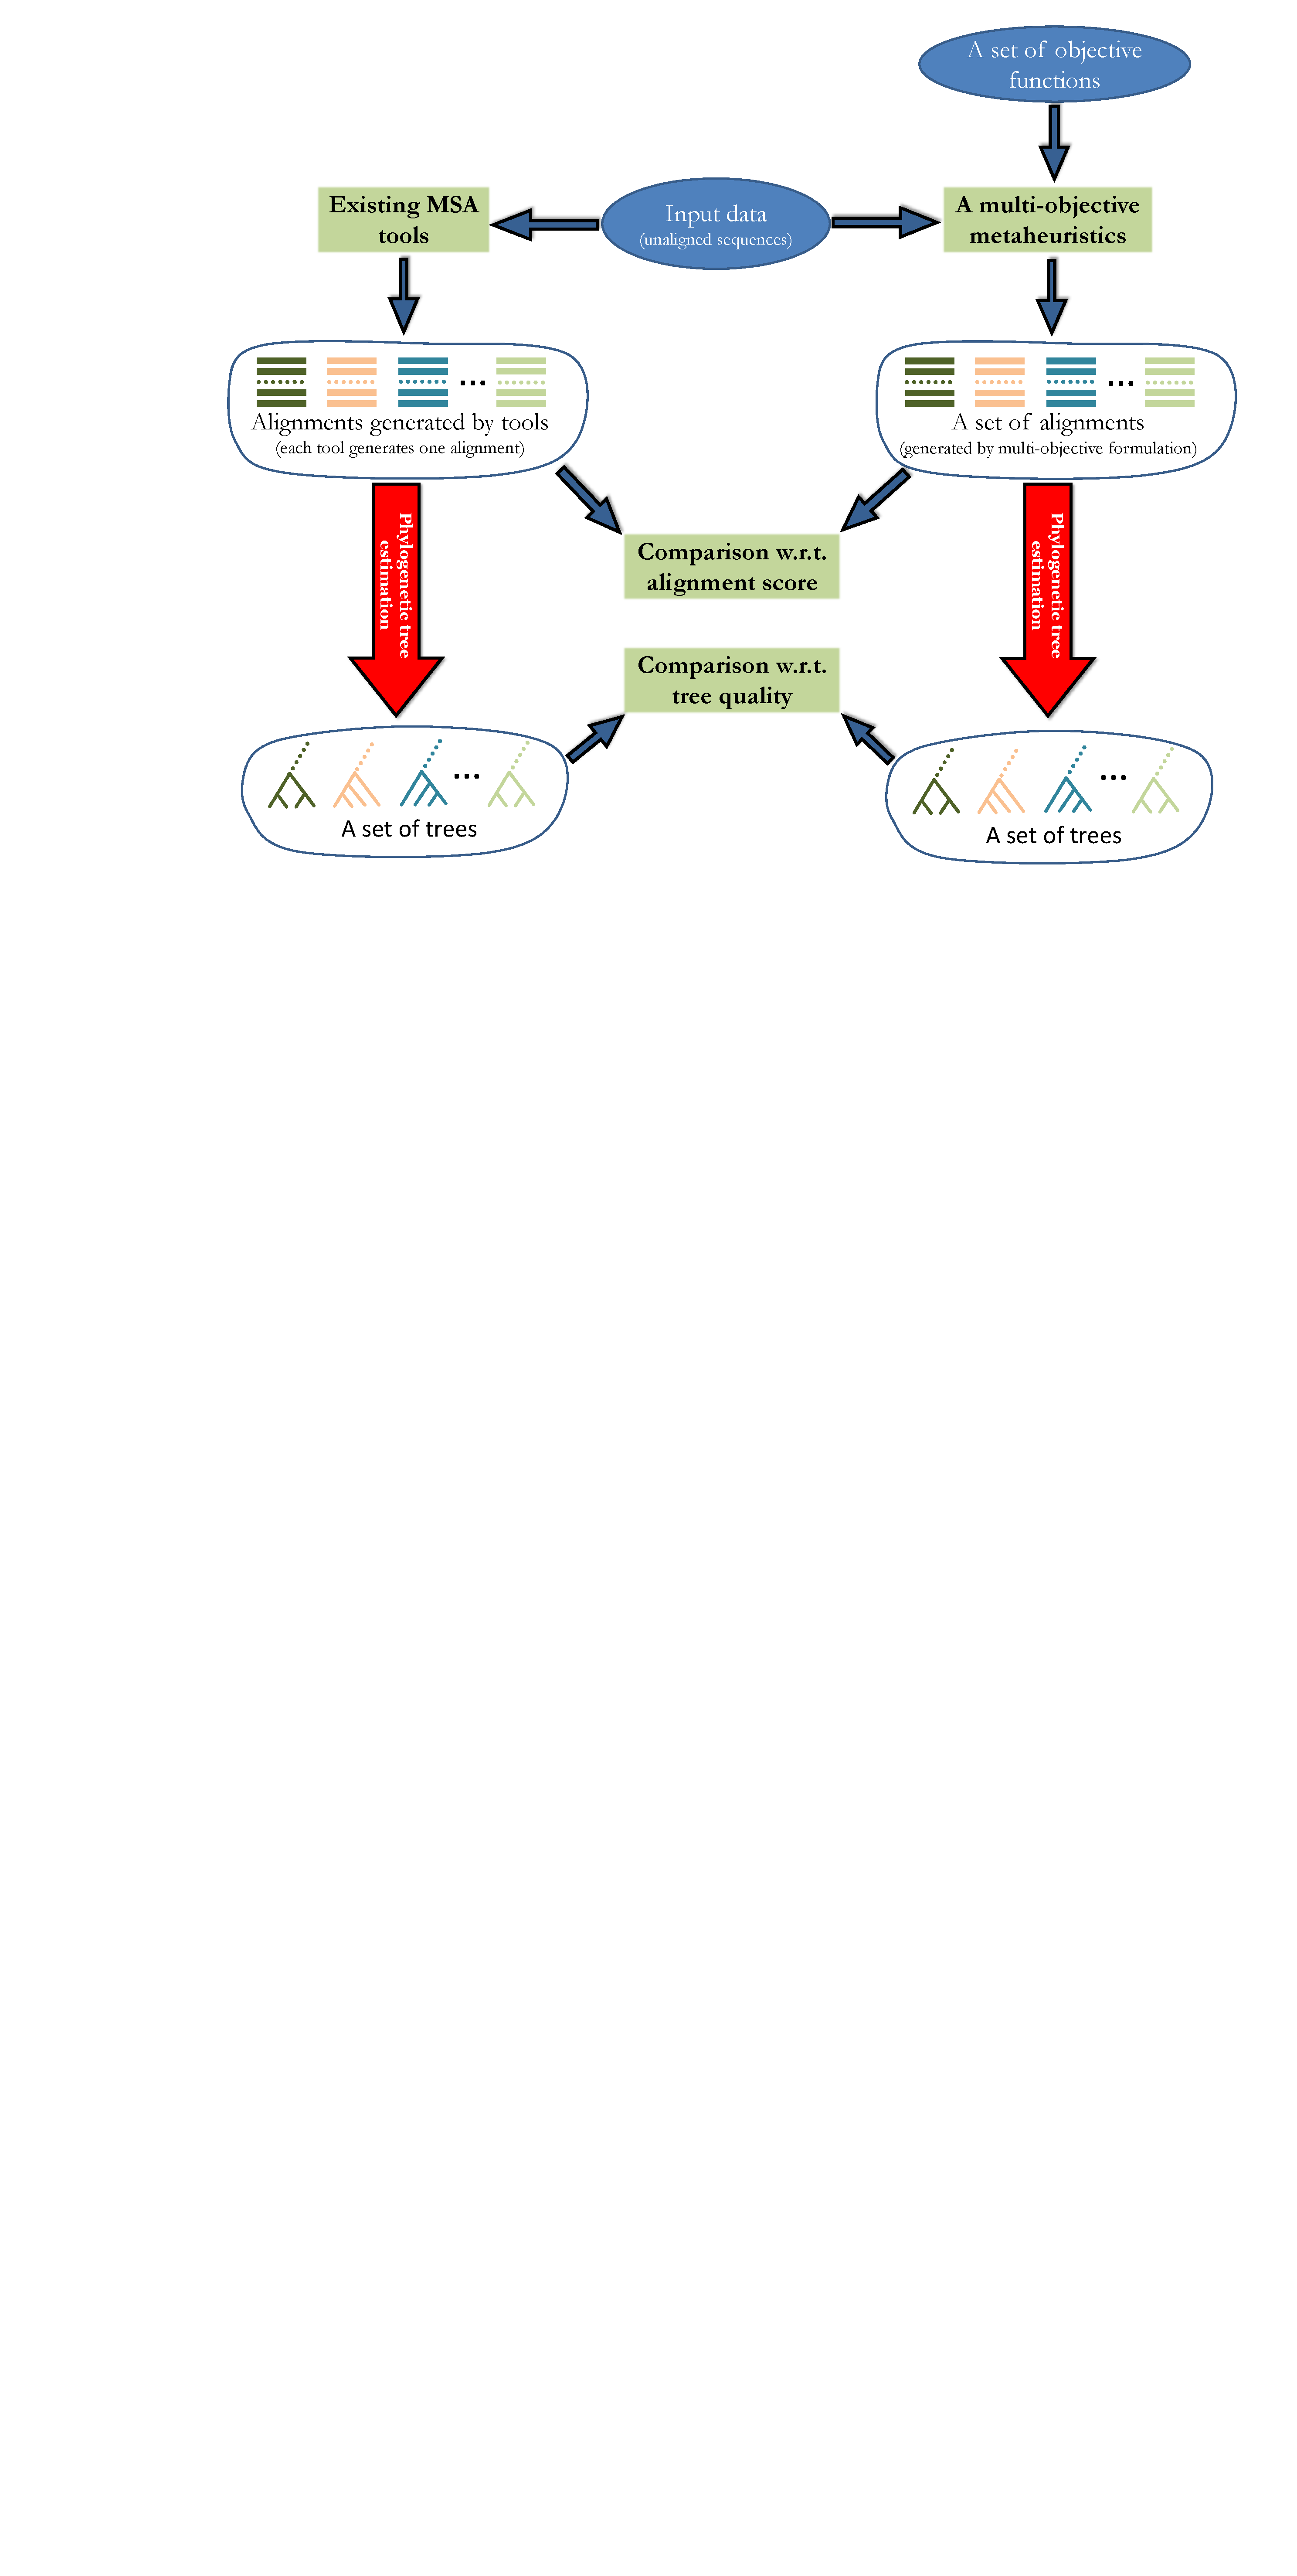
\includegraphics[width=2\columnwidth]{Figure/pipeline}
	\caption{Our methodology for finding the impact of a multi-objective formulation (i.e., a set of objective functions) of MSA on phylogenetic tree estimation. For each dataset (i.e., unaligned sequences), we run an multi-objective metaheuristics. It simultaneously optimizes the given objective functions and outputs a set of alignments which represents the best-possible compromise among all objective functions. We also run several existing MSA tools on that dataset and each tool generates one alignment. We evaluate the quality of each generated alignments with respect to the reference alignments using widely used scores. Also we estimate phylogenetic trees for all alignments and evaluate each tree with respect to the reference. Then we compare the alignments and the corresponding phylogenetic trees generated by the multi-objective formulation with the ones generated by the existing tools based on alignment score as well as tree quality. We also observe the association between alignment scores and tree quality values to examine whether it is appropriate to use alignment score in the context of phylogeny estimation.}
	\label{fig:pipeline}
\end{figure*}

%In this section, we discuss our experimental results on both simulated and biological datasets. We conduct extensive experiments with 10 replicates of 100-taxon simulated dataset, two biological rRNA datasets and 27 BAliBASE datasets. We begin by picking two sets of objective functions by analyzing the generated set of alignments based on resultant tree quality. Then for all datasets we compare the alignments generated by those objective sets with nine state-of-the-art tools. 

We conducted extensive experiments with 10 replicates of 100-taxon simulated dataset, two biological rRNA datasets and 27 BAliBASE datasets. We begin by carefully and systematically selecting two multi-objective formulations which are potentially useful for phylogenetic tree estimation. Then for each dataset, we generate alignments through running multi-objective metaheuristics as well as nine state-of-the-art MSA tools. Then we compare those alignments with respect to both generic and domain specific quality measures. In this section, we discuss our obtained results after a brief discussion on our experimental design and datasets. In what follows, unless otherwise specified, when we discuss the (best) results of a tool, we mean one of the above-mentioned nine tools.

\subsection{Experimental design}
Our experimental methodology is briefly described below (see also Figure~\ref{fig:pipeline}):
\begin{itemize}
	\item \underline{Step 1:} Following a systematic approach involving multiple linear regression applied on a simulated dataset, we first make an attempt to identify and choose two multi-objective formulations that turn out to be potentially more effective in the context of phylogeny estimation. 
	\item \underline{Step 2:} We run a popular and effective multi-objective metaheuristics on both biological and simulated datasets to optimize each set of objective functions selected in Step 1. Each run of the meteheuristics on each dataset gives us a set of alignments as output. 
	\item \underline{Step 3:} We also run nine state-of-the-art MSA tools (see Section~\ref{sec:methods}, Table~\ref{tab:msa_tools}) \commentA{with default parameters} to generate alignments on all these datasets.
	% and then estimate maximum likelihood (ML) phylogenetic tree from those alignments. We evaluate the quality of these alignments and ML trees.
	\item \underline{Step 4:} We evaluate the quality of each generated alignment with respect to the reference alignment using two popular measures, namely, SP score and TC score. 
	%For biological datasets, we used manually curated alignments as reference.
	\item \underline{Step 5:} For each of the generated alignments, we infer maximum likelihood (ML) phylogenetic tree. Then we measure the quality of each inferred tree with respect to the reference tree (true tree) using the mostly used measure in the literature called false negative (FN) rate.
	\item \underline{Step 6:} Finally we closely compare the alignments and the corresponsing ML trees generated by the multi-objective optimization with the ones generated by the state-of-the-art tools. % using statistical measures.
\end{itemize}


\subsection{Datasets}
%We aim to validate the effectiveness of an objective function in terms of how it can help to estimate phylogenetic tree. So, in this context a good objective function has good statistical evidence of leading to good trees. To conduct our study we require knowledge of the true phylogenetic tree which can be used as a reference for measuring the goodness of estimated trees. 
To conduct our study, we choose three different categories of datasets: 100-taxon simulated dataset, Biological rRNA datasets and BAliBASE datasets. We use the 100-taxon simulated dataset for dual purposes. At first, we conduct experiments with this dataset to examine whether a multi-objective formulation of MSA is potentially phylogeny-aware and in the sequel, we select two such formulations. Afterwards, we validate the effectiveness of these formulations against the state-of-the-art MSA tools based on this dataset as well as other biological datasets. We now introduce each of these datasets.
% We now briefly introduce them in this subsection.   

\subsubsection{100-taxon simulated dataset}
We used 10 (out of 20) randomly selected replicates (R0, R2, R4, R6, R9, R10, R13, R14, R17, R19) of simulated nucleotide dataset from the study of~\citealp{liu2009rapid}. It is publicly available at \url{https://sites.google.com/eng.ucsd.edu/datasets/sate-i}. Table~\ref{tab:sim_stat} gives the reference alignment statistics.
% generated from a model tree (can be used as true tree) with model condition (100 taxa, short gap length type)

% Table generated by Excel2LaTeX from sheet 'Sheet1'
\begin{table}[htbp]
	\centering
	\caption{Reference alignments for 100-taxon simulated dataset.}
	   \begin{tabular}{|l|r|}
		\hline
		\multicolumn{1}{|c|}{Feature} & \multicolumn{1}{c|}{Value} \\
		\hline
		Number of taxa & 100 \\
		\hline
		Number of sites & 1698.2 \\
		\hline
		Percent indels & 40.4 \\
		\hline
		Avg. gap length & 3.1 \\
		\hline
		\end{tabular}%
	\label{tab:sim_stat}%
\end{table}%


\subsubsection{Biological rRNA datasets}
We analyzed two biological ribosomal RNA datasets, 23S.E and 23S.E.aa\_ag, from~\citealp{liu2009rapid} which are challenging for phylogeny estimation methods. Each of these datasets is given with a highly reliable, curated reference alignment from Gutell Lab. The statistics of the reference alignments are summarized in Table~\ref{tab:bio_stat}. Reference trees for these datasets were generated from the reference alignments by running RAxML~\citep{stamatakis2014raxml} with bootstrapping, and retaining only the highly supported edges. We evaluated generated alignments with respect to the reference alignment using the tool FastSP \citep{mirarab2011fastsp}.

% Table generated by Excel2LaTeX from sheet 'Sheet2'
\begin{table}[htbp]
	\small
	\centering
	\caption{Reference alignments for two biological rRNA datasets.}
	\begin{tabular}{|l|r|r|}
		\hline
		\multicolumn{1}{|c|}{Feature} & \multicolumn{1}{c|}{23S.E.aa\_ag} & \multicolumn{1}{c|}{23S.E} \\
		\hline
		Number of taxa & 144   & 117 \\
		\hline
		Number of sites & 8,619 & 9,079 \\
		\hline
		Percent indels & 61.1  & 59.7 \\
		\hline
		Avg. gap length & 13.5  & 12.6 \\
		\hline
	\end{tabular}%
	\label{tab:bio_stat}%
\end{table}%

\subsubsection{BAliBASE datasets}
BAliBASE 3.0 \citep{thompson2005balibase} is the most widely used benchmark alignment databases of protein families. It provides manually refined reference alignments of high quality based on 3D structural superposition. These datasets are organized into six groups according to their families and similarities: \commentA{RV11 (very divergent sequences, residue identity below 20\% ), RV12 (medium to divergent sequences, 20\%-40\% residue identity), RV20 (families with one or more highly divergent sequences), RV30 (divergent subfamilies), RV40 (sequences with large terminal N/C extensions), and RV50 (sequences with large internal insertions).} In this study, we selected four to five representative datasets from each group as shown in Table~\ref{tab:balibase}. We generated reference trees for these datasets by running RAxML with bootstrapping. We evaluated estimated alignments with respect to the core blocks (regions for which reliable alignments are known to exist) using the program bali\_score available at~\url{http://www.lbgi.fr/balibase/BalibaseDownload/}.
% We randomly take 27 (out of 218) datasets (Table~\ref{tab:balibasel})

% Table generated by Excel2LaTeX from sheet 'Sheet2'
\begin{table}[htbp]
	\small
	\centering
	\caption{ BAliBASE datasets selected for this study.}
	\begin{tabular}{|l|L{5.1cm}|}
		\hline
		\multicolumn{1}{|c|}{Group} & \multicolumn{1}{c|}{Datasets selected} \\
		\hline
		RV11  & BB11005, BB11018, BB11020, BB11033 \\
		\hline
		RV12  & BB12001, BB12013, BB12022, BB12035, BB12044 \\
		\hline
		RV20  & BB20001, BB20010, BB20022, BB20033, BB20041 \\
		\hline
		RV30  & BB30002, BB30008, BB30015, BB30022 \\
		\hline
		RV40  & BB40001, BB40013, BB40025, BB40038, BB40048 \\ %
		\hline
		RV50  & BB50001, BB50005, BB50010, BB50016 \\
		\hline
	\end{tabular}%
	\label{tab:balibase}%
\end{table}%

\subsection{Selection of multi-objective formulations}
%We choose two sets of objective functions (i.e. multi-objective formulation) to conduct experiments based on this dataset. We select the first set of objective functions from among three existing studies based on their relative performance in the context of phylogeny estimation. Afterwards, we follow a similar approach to form the second set by incorporating our proposed objective functions. Now we discuss the selection process of these two sets along with their performance on this dataset.
As has been mentioned above, we have used 100-taxon simulated dataset for dual purposes: to select one or more multi-objective formulations that have the potential to be `phylogeny-aware' (Section~\ref{sec:existing_msa_formulation}, \ref{sec:new_msa_formulation}) and to judge the efficacy of the detected formulations in comparison with the other state-of-the-art tools (Section~\ref{sec:result_100_taxon}). We first conduct extensive experiments to choose a formulation (i.e., a set of objective functions) of MSA from among the existing popular ones from the literature (Section~\ref{sec:existing_msa_formulation}); subsequently, we also suggest a new promising formulation (Section~\ref{sec:new_msa_formulation}).  
%We use this dataset to select a potentially phylogeny-aware multi-objective formulation (i.e., a set of objective functions) of MSA from the literature. Then based on the same dataset we present a new promising formulation. We perform these steps by adopting a novel methodology based on the careful application of multiple linear regression. Now we discuss the selection process of these two formulations followed by their performance against the state-of-the-art tools.
%At the end, we compare these two objective set based on their performance on 10 replicates.
\begin{figure*}[!htbp]	
	\begin{adjustwidth}{-1cm}{-1cm}
	\centering
	\begin{subfigure}{0.35\textwidth}
		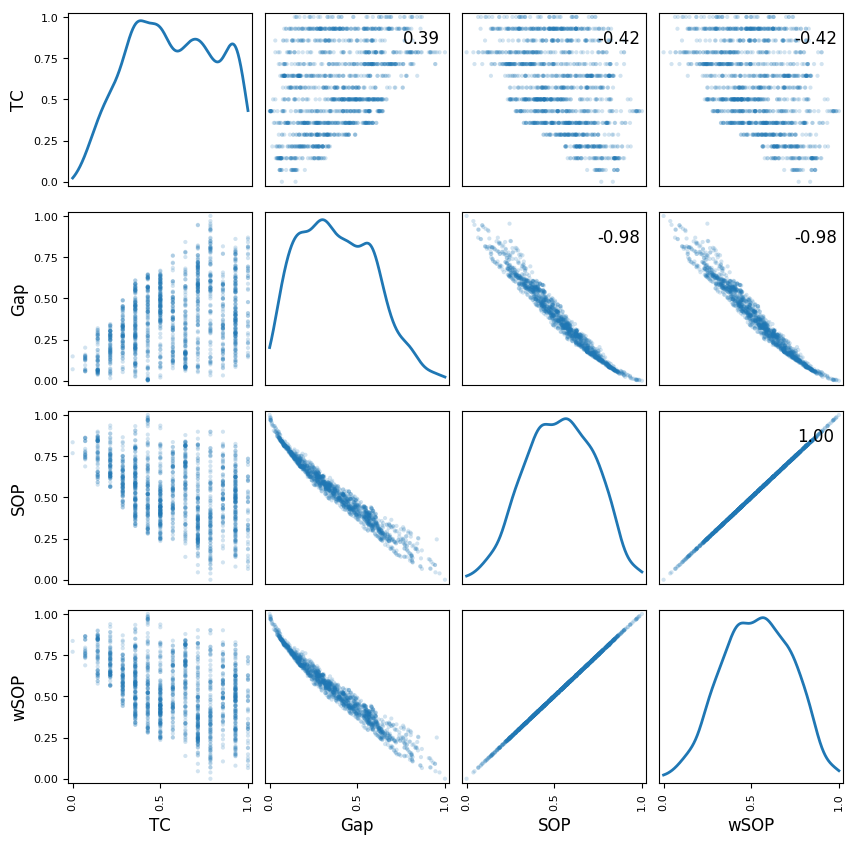
\includegraphics[width=\columnwidth]{Figure/NumGaps_SOP_TC_wSOP/precomputedInit/R0/fig/scatter_mattrix}
		\caption{R0}
		%\label{fig:con_pr09}
	\end{subfigure}	
	\begin{subfigure}{0.35\textwidth}
		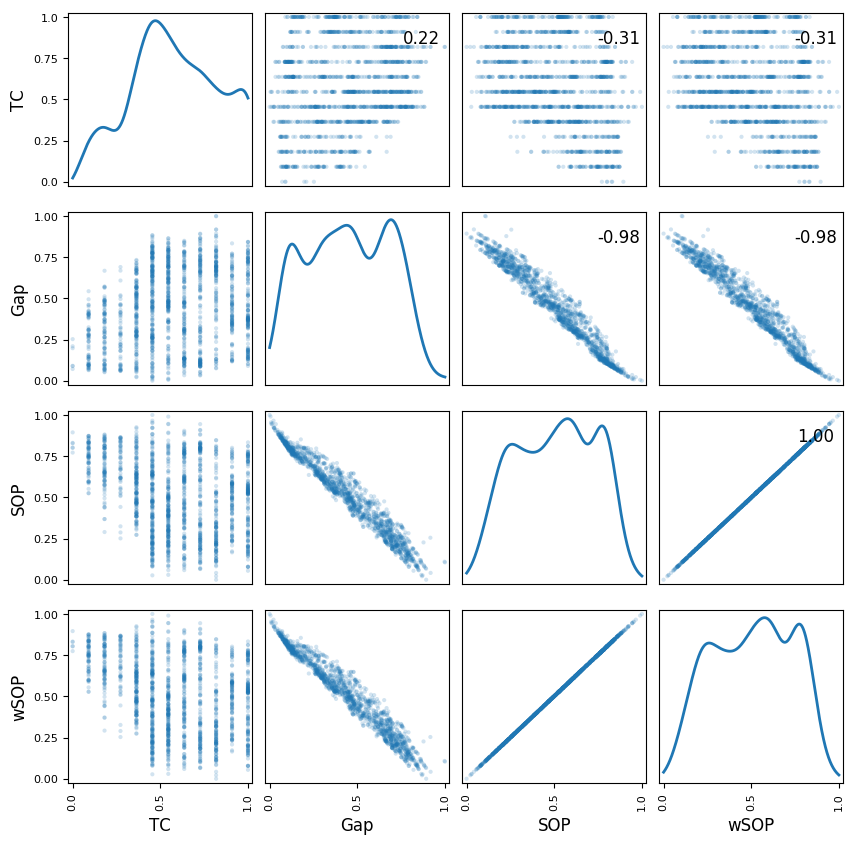
\includegraphics[width=\columnwidth]{Figure/NumGaps_SOP_TC_wSOP/precomputedInit/R4/fig/scatter_mattrix}
		\caption{R4}
		%\label{fig:con_pr09}
	\end{subfigure}
	\begin{subfigure}{0.35\textwidth}
		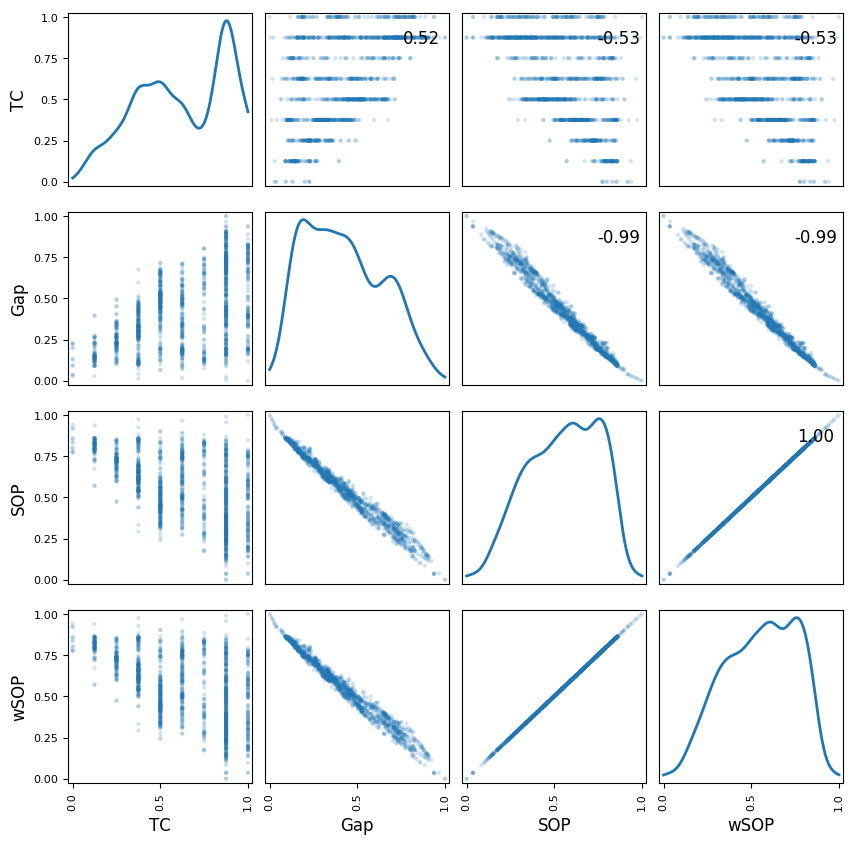
\includegraphics[width=\columnwidth]{Figure/NumGaps_SOP_TC_wSOP/precomputedInit/R9/fig/scatter_mattrix}
		\caption{R9}
		%\label{fig:con_pr09}
	\end{subfigure}
	\begin{subfigure}{0.35\textwidth}
		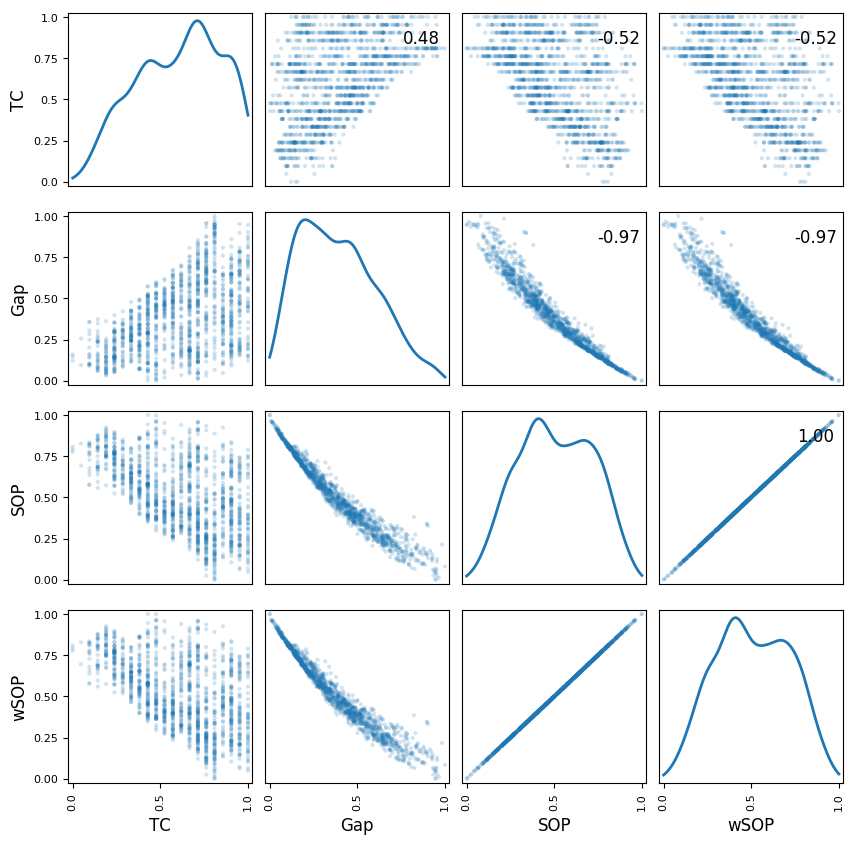
\includegraphics[width=\columnwidth]{Figure/NumGaps_SOP_TC_wSOP/precomputedInit/R14/fig/scatter_mattrix}
		\caption{R14}
		%\label{fig:con_pr09}
	\end{subfigure}
	\begin{subfigure}{0.35\textwidth}
		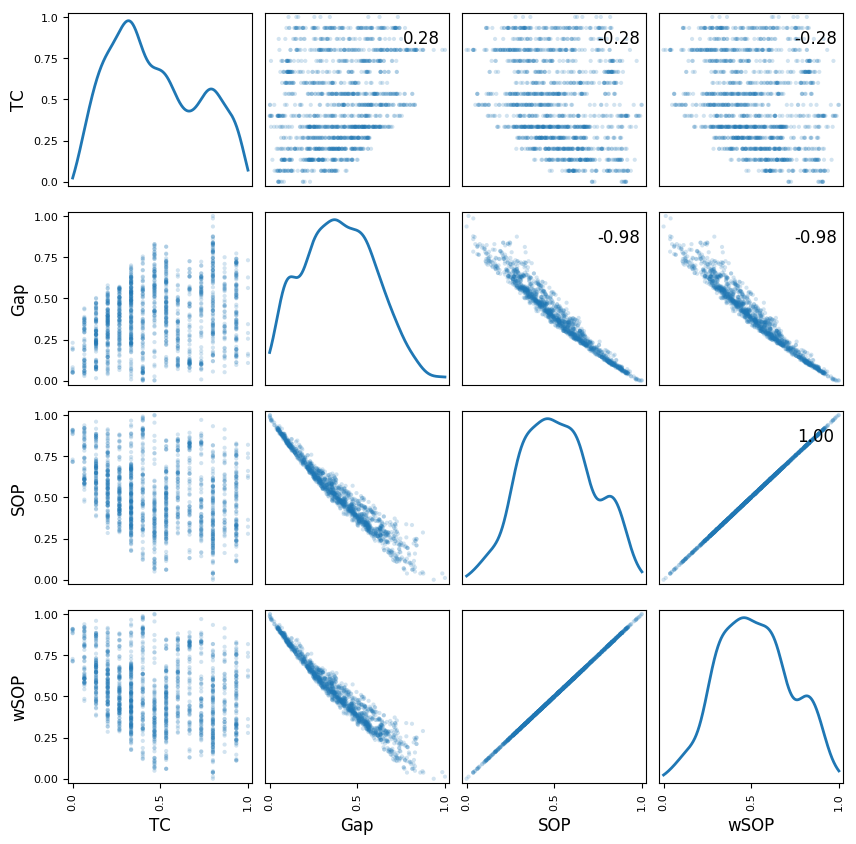
\includegraphics[width=\columnwidth]{Figure/NumGaps_SOP_TC_wSOP/precomputedInit/R19/fig/scatter_mattrix}
		\caption{R19}
		%\label{fig:con_pr09}
	\end{subfigure}
	\caption{Scatter-plot matrices depicting the pairwise relationship of all objective functions on five randomly selected replicates. We turn each objective function into minimization form and then normalize using min-max technique. In each matrix, the diagonal cells show the distribution of objective values (estimated using KDE) while the non-diagonal cells show the correlation between pairs of objective functions. Each upper-diagonal cell contains the value of correlation coefficient $r$ between the corresponding pair of objective functions.}
	\label{fig:nature_obj}
	\end{adjustwidth}
\end{figure*}

\begin{figure*}[!htbp]
	\centering
	\small
	\begin{adjustwidth}{-1cm}{-1cm}
		\begin{tabular}{l||C{0.24\textwidth}|C{0.24\textwidth}|C{0.24\textwidth}|C{0.24\textwidth} }
			& TC & Gap & SOP & wSOP\\\hline\hline
			\rotatebox[origin=c]{-90}{R0} & 
			\raisebox{-.5\height}{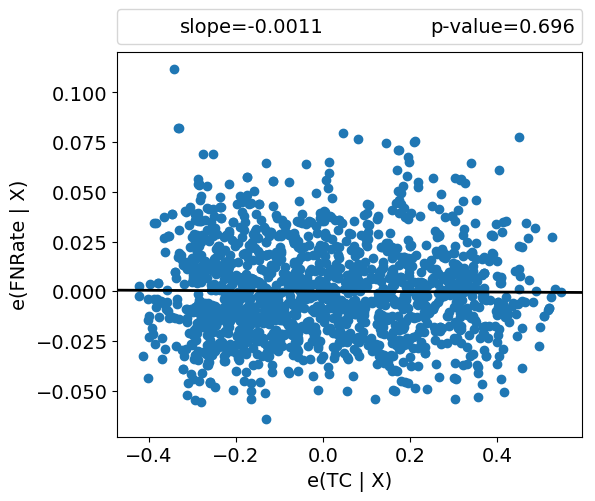
\includegraphics[width=0.25\textwidth]{Figure/NumGaps_SOP_TC_wSOP/precomputedInit/R0/fig/tc_partial_regression}} &
			\raisebox{-.5\height}{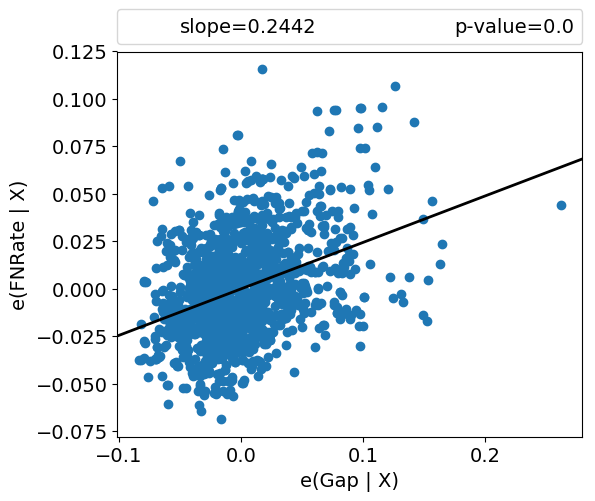
\includegraphics[width=0.25\textwidth]{Figure/NumGaps_SOP_TC_wSOP/precomputedInit/R0/fig/gap_partial_regression}} & 
			\raisebox{-.5\height}{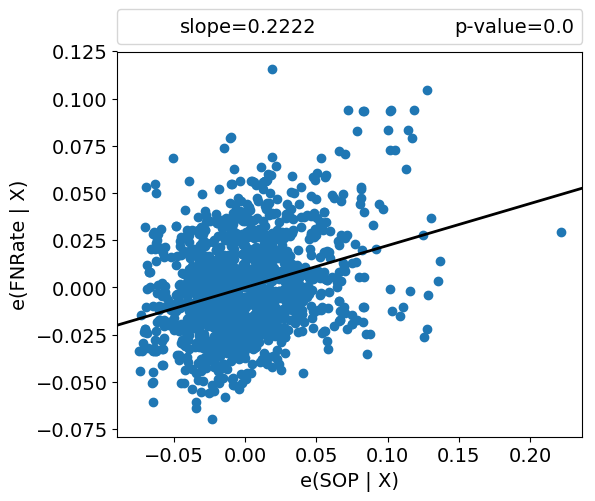
\includegraphics[width=0.25\textwidth]{Figure/NumGaps_SOP_TC_wSOP/precomputedInit/R0/fig/sop_partial_regression}} & 
			\raisebox{-.5\height}{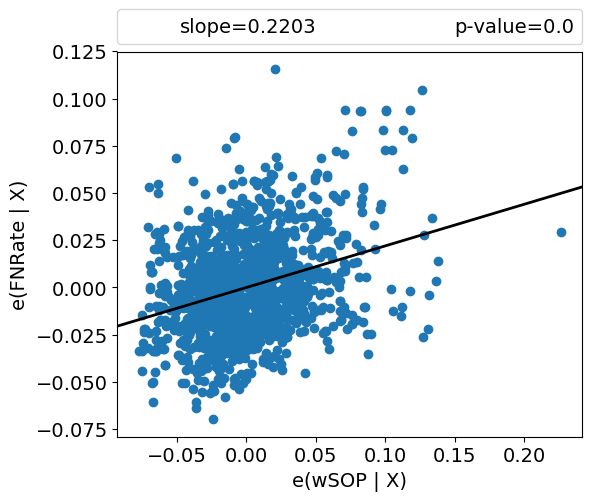
\includegraphics[width=0.25\textwidth]{Figure/NumGaps_SOP_TC_wSOP/precomputedInit/R0/fig/wsop_partial_regression}} 	
			\\\hline
			\rotatebox[origin=c]{-90}{R4} &
			\raisebox{-.5\height}{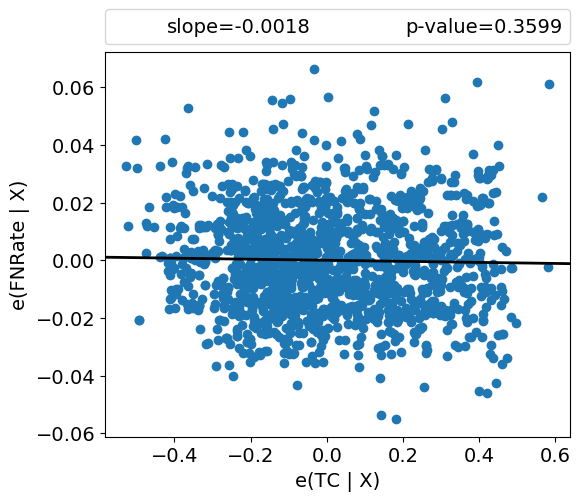
\includegraphics[width=0.25\textwidth]{Figure/NumGaps_SOP_TC_wSOP/precomputedInit/R4/fig/tc_partial_regression}} &
			\raisebox{-.5\height}{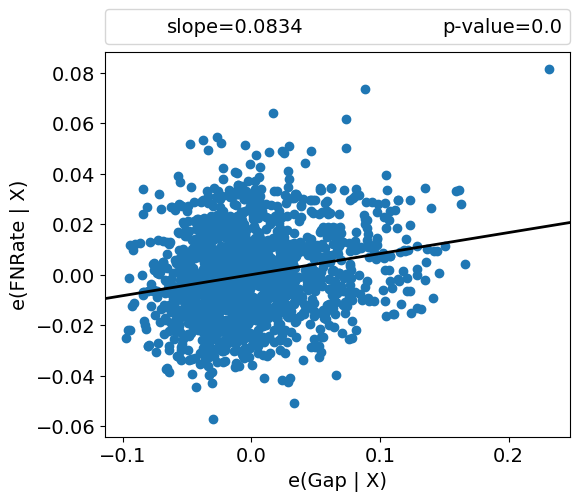
\includegraphics[width=0.25\textwidth]{Figure/NumGaps_SOP_TC_wSOP/precomputedInit/R4/fig/gap_partial_regression}} & 
			\raisebox{-.5\height}{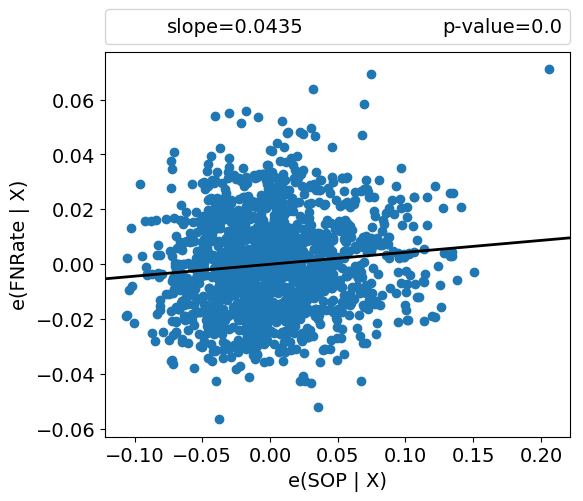
\includegraphics[width=0.25\textwidth]{Figure/NumGaps_SOP_TC_wSOP/precomputedInit/R4/fig/sop_partial_regression}} & 
			\raisebox{-.5\height}{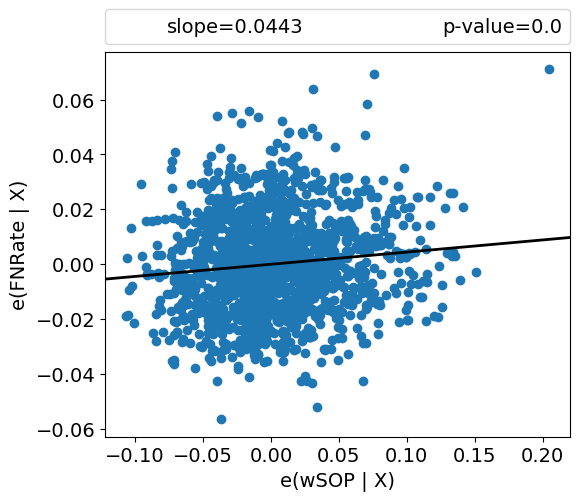
\includegraphics[width=0.25\textwidth]{Figure/NumGaps_SOP_TC_wSOP/precomputedInit/R4/fig/wsop_partial_regression}}
			\\\hline
			\rotatebox[origin=c]{-90}{R9} &
			\raisebox{-.5\height}{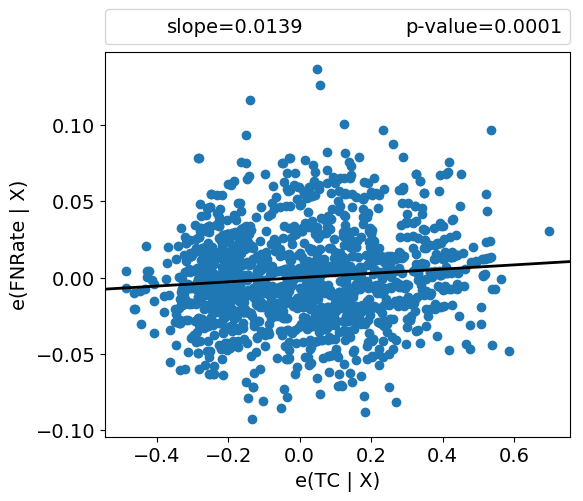
\includegraphics[width=0.25\textwidth]{Figure/NumGaps_SOP_TC_wSOP/precomputedInit/R9/fig/tc_partial_regression}} &
			\raisebox{-.5\height}{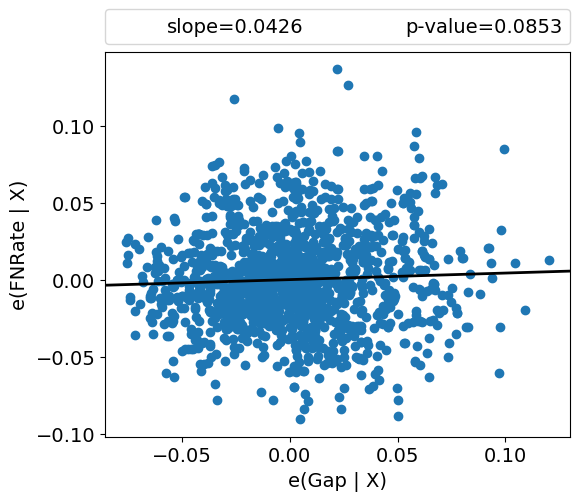
\includegraphics[width=0.25\textwidth]{Figure/NumGaps_SOP_TC_wSOP/precomputedInit/R9/fig/gap_partial_regression}} & 
			\raisebox{-.5\height}{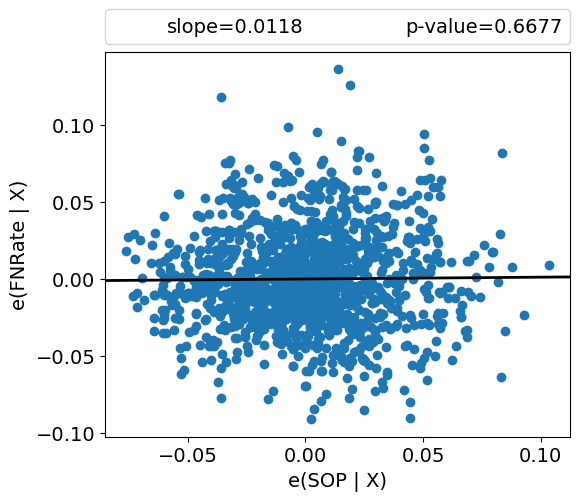
\includegraphics[width=0.25\textwidth]{Figure/NumGaps_SOP_TC_wSOP/precomputedInit/R9/fig/sop_partial_regression}} & 
			\raisebox{-.5\height}{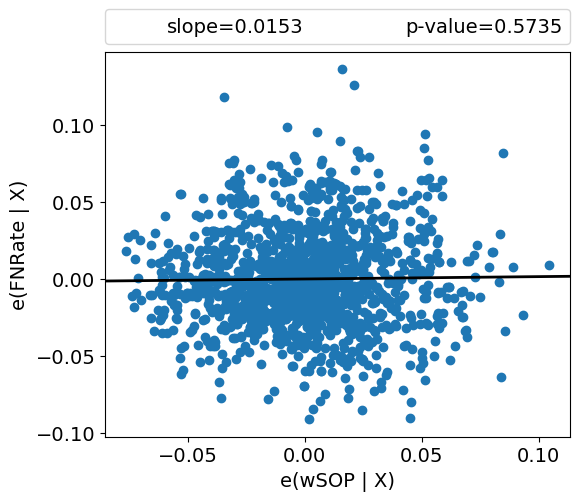
\includegraphics[width=0.25\textwidth]{Figure/NumGaps_SOP_TC_wSOP/precomputedInit/R9/fig/wsop_partial_regression}}
			\\\hline
			\rotatebox[origin=c]{-90}{R14} &
			\raisebox{-.5\height}{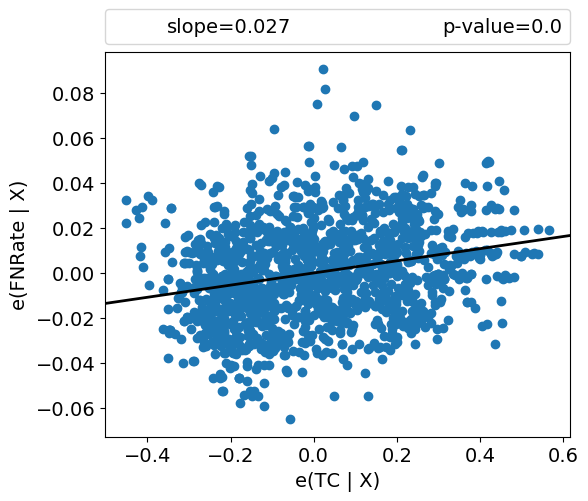
\includegraphics[width=0.25\textwidth]{Figure/NumGaps_SOP_TC_wSOP/precomputedInit/R14/fig/tc_partial_regression}} &
			\raisebox{-.5\height}{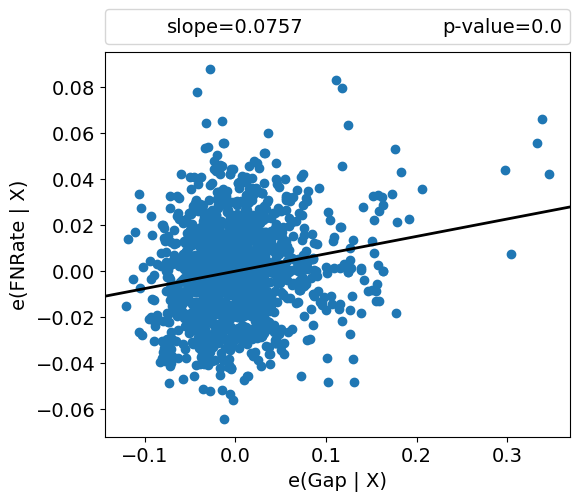
\includegraphics[width=0.25\textwidth]{Figure/NumGaps_SOP_TC_wSOP/precomputedInit/R14/fig/gap_partial_regression}} & 
			\raisebox{-.5\height}{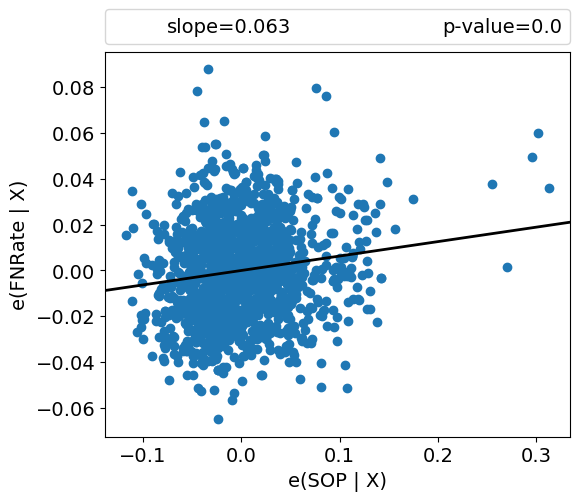
\includegraphics[width=0.25\textwidth]{Figure/NumGaps_SOP_TC_wSOP/precomputedInit/R14/fig/sop_partial_regression}} & 
			\raisebox{-.5\height}{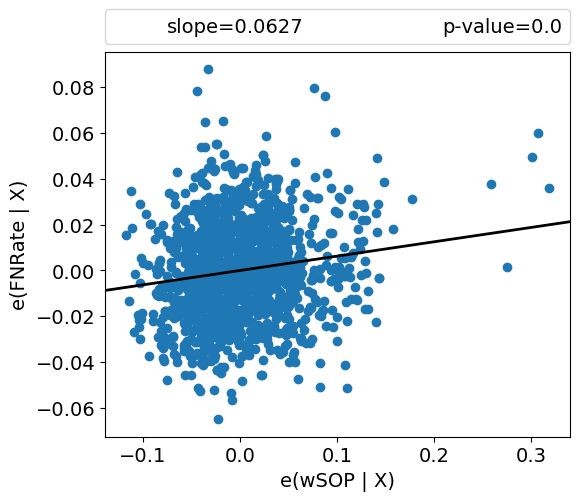
\includegraphics[width=0.25\textwidth]{Figure/NumGaps_SOP_TC_wSOP/precomputedInit/R14/fig/wsop_partial_regression}}
			\\\hline
			\rotatebox[origin=c]{-90}{R19} &
			\raisebox{-.5\height}{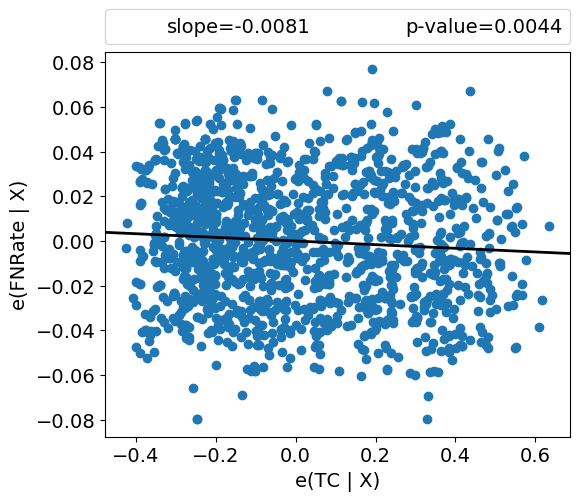
\includegraphics[width=0.25\textwidth]{Figure/NumGaps_SOP_TC_wSOP/precomputedInit/R19/fig/tc_partial_regression}} &
			\raisebox{-.5\height}{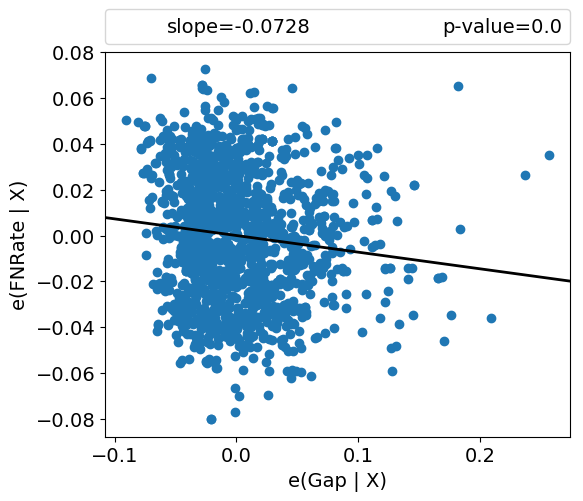
\includegraphics[width=0.25\textwidth]{Figure/NumGaps_SOP_TC_wSOP/precomputedInit/R19/fig/gap_partial_regression}} & 
			\raisebox{-.5\height}{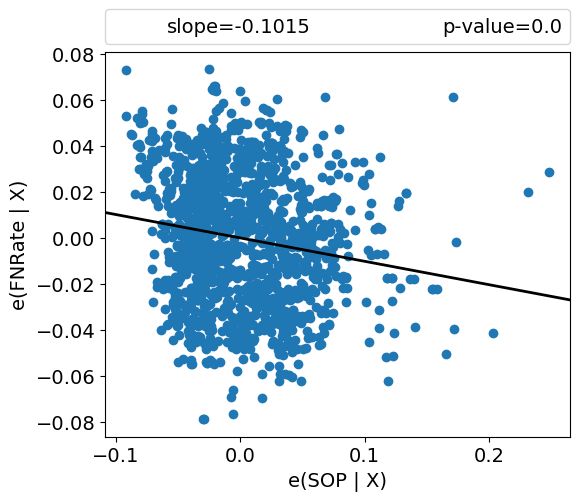
\includegraphics[width=0.25\textwidth]{Figure/NumGaps_SOP_TC_wSOP/precomputedInit/R19/fig/sop_partial_regression}} & 
			\raisebox{-.5\height}{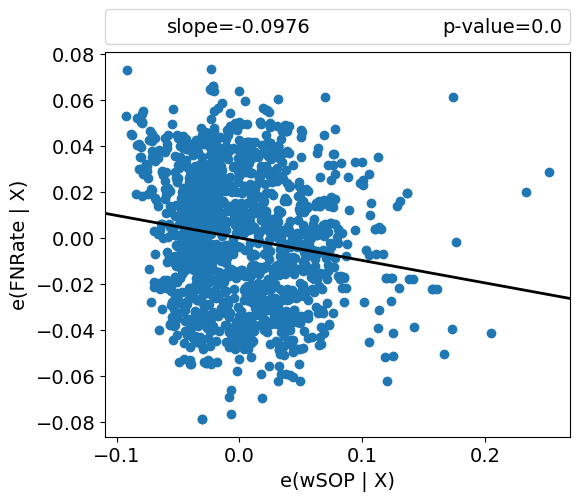
\includegraphics[width=0.25\textwidth]{Figure/NumGaps_SOP_TC_wSOP/precomputedInit/R19/fig/wsop_partial_regression}}
			\\\hline
		\end{tabular}
	\caption{Multiple linear regression model for identifying the association among FN rate and three objective functions (TC, Gap and SOP/wSOP) fitted to five randomly selected replicates. There is one figure for each possible combination (replicate, objective function). Each partial regression plot shows the association between an objective function and FN rate while holding the remaining two objectives constant. In a plot for an objective function $ OF $, the horizontal axis, $e(OF|X)$, denotes the residuals from regressing $OF$ against the remaining objective functions and the vertical axis, $e(FNRate|X)$, denotes the residuals from regressing FN rate against all the objective functions except $ OF $.} 
	\label{fig:mul_lin_reg}
	\end{adjustwidth}
\end{figure*}

\begin{figure*}[!htbp]
	\centering
	\begin{adjustwidth}{-1cm}{-1cm}
	\begin{subfigure}{0.22\textwidth}
		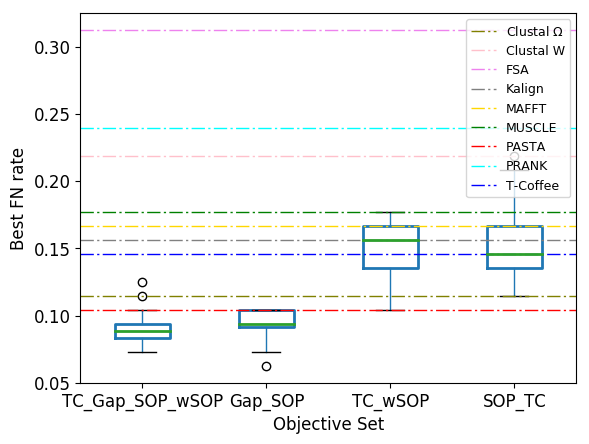
\includegraphics[width=\columnwidth]{Figure/summary/precomputedInit/R0/objset_fnrate_rank}
		\caption{R0}
		%\label{fig:con_pr09}
	\end{subfigure}	
	\begin{subfigure}{0.22\textwidth}
		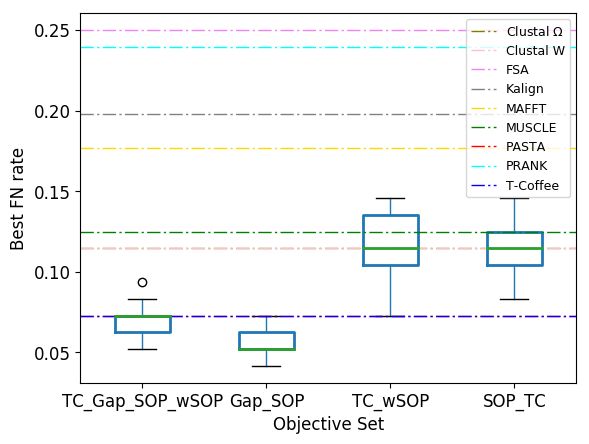
\includegraphics[width=\columnwidth]{Figure/summary/precomputedInit/R4/objset_fnrate_rank}
		\caption{R4}
		%\label{fig:con_pr09}
	\end{subfigure}
	\begin{subfigure}{0.22\textwidth}
		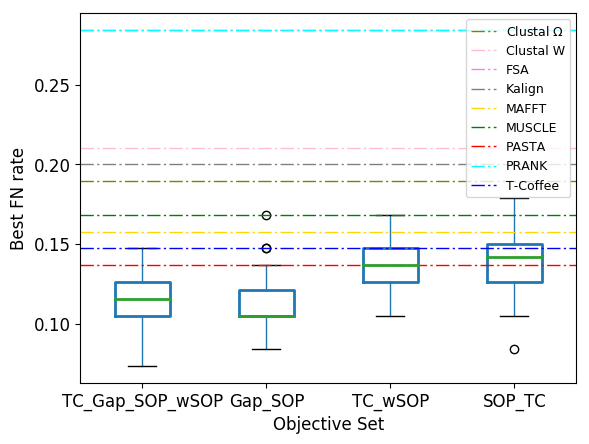
\includegraphics[width=\columnwidth]{Figure/summary/precomputedInit/R9/objset_fnrate_rank}
		\caption{R9}
		%\label{fig:con_pr09}
	\end{subfigure}
	\begin{subfigure}{0.22\textwidth}
		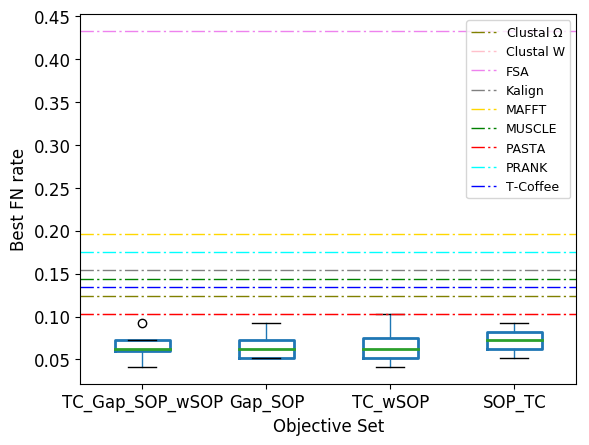
\includegraphics[width=\columnwidth]{Figure/summary/precomputedInit/R14/objset_fnrate_rank}
		\caption{R14}
		%\label{fig:con_pr09}
	\end{subfigure}
	\begin{subfigure}{0.22\textwidth}
		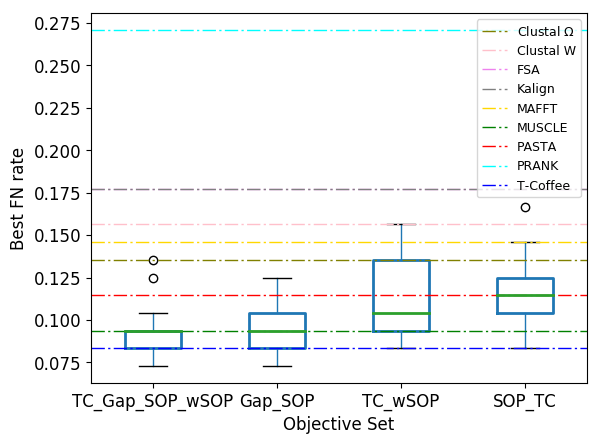
\includegraphics[width=\columnwidth]{Figure/summary/precomputedInit/R19/objset_fnrate_rank}
		\caption{R19}
		%\label{fig:con_pr09}
	\end{subfigure}
	\caption{Comparison among objective sets based on the distribution of the collection of the best FN rates from each run. The performance of the state-of-the-art tools are shown using horizontal lines.}
	\label{fig:rank_best_fn_rate}
\end{adjustwidth}
\end{figure*}
\subsubsection{Selection from among the existing formulations}
\label{sec:existing_msa_formulation}
To reduce the computational effort, we pre-select three multi-objective formulations of MSA and limit our investigation thereon. Thus we choose one of the formulations from among \{Gap, SOP\}~\citep{abbasi2015local}, \{SOP, TC\}~\citep{da2010alineaga} and \{wSOP, TC\}~\citep{rubio2016bee, rubio2016hybrid} (see Section~\ref{sec:methods} Table~\ref{tab:abbr}). We experiment with five randomly selected replicates (R0, R4, R9, R14, R19) and then judge based on two criteria: firstly, we used multiple linear regression analysis to examine the association between individual objective function and FN rate; secondly, we assess the alignments generated through the optimization of each set of objective functions in terms resultant ML trees. 

We need to consider the relationship between each pair of objective functions to properly interpret the result of multiple linear regression. We perform this by running an appropriate multi-objective metaheuristic (i.e., NSGA-III~\citep{deb2014evolutionary}) for 25 times which optimizes all the objective functions (i.e., \{Gap, SOP, wSOP, TC\})  and thus we obtain a large collection of diverse alignments. We visualize the interrelations among the objective values of those solutions using a $ 4\times4 $ scatter-plot matrix~\cite{kalyanmoy2001multi} as shown in Figure~\ref{fig:nature_obj}. Here each diagonal cell of a matrix depicts the distribution of the values of an objective function estimated using Kernel Density Estimation (KDE) and the non-diagonal cells show the correlation between each pair of objective functions. As our metaheuristic aalgorithm tries to minimize all objective functions, we treat the maximization objective values by multiplying with -1. In the sequel, we normalize all the objective values using min-max technique and as such the maximization objectives are turned into minimization ones. From these scatter-plot matrices, we have the follwoing two key observations.
\begin{enumerate}[(a)]
	
	\item In all the cases, SOP is totally correlated with wSOP. So we do not need to optimize both of them. Moreover, this high correlation creates a serious problem in multiple regression analysis called multicollinearity~\citep{montgomery2012introduction}. Therefore, we should not keep these two objective functions together in our regression analysis. Also it is redundant to considering both of them in the multi-objective formulation. 
	
	\item SOP is clearly in conflict with Gap across all the replicates. Therefore, if we optimize them simultaneously, we can generate many diverse solutions which represent the compromise between these two objective functions~\citep{kalyanmoy2001multi}. These diverse collection is likely to contain the desired alignment for any kind of dataset.
	
\end{enumerate}

As the objective functions are inter-related, we need to measure the degree of association between an objective and FN rate while holding the remaining objectives constant to avoid getting any spurious result~\citep{montgomery2012introduction}. Therefore, we perform multiple linear regression by employing the following model:
\begin{equation}
\small
\begin{split}
\text{FN rate} = \beta_0 + \beta_1 \times \text{TC}+ \beta_2 \times \text{Gap} + \\
\beta_3 \times \text{SOP (or wSOP)} + \epsilon \label{eq:multi_lin_reg}
\end{split}
\end{equation}

Each coefficient ($\beta_1, \beta_2$ and $\beta_3$) represents the expected change in the FN rate per unit change in the corresponding objective function when all the remaining objective functions are held constant. For this reason they ($\beta_i$) are called partial regression coefficients. $\epsilon$ is the random error component which is assumed to follow a Gaussian distribution with mean zero and some fixed standard deviation. We fit this model to the solutions generated by optimizing the set \{Gap, SOP, wSOP, TC\}. For each of those solutions, we estimate ML tree and evaluate its quality in terms of FN rate.  We estimate these coefficients using least-squares method and illustrate them using partial regression plots~\citep{montgomery2012introduction} in Figure~\ref{fig:mul_lin_reg}. We apply $t$-test on individual regression coefficient (i.e., slope) $\beta_i$ (with null hypothesis $\beta_i=0$) to test the significance of that association. The test results (slope, $p$-value) are incorporated in the figure. We can note the following two interesting points from these results.
\begin{enumerate}[(a)]
	\item In majority of the cases (R0, R4 and R14), Gap, SOP and wSOP exhibit a good degree of association with FN rate (i.e positive slope) with high confidence (p-value close to 0) compared to other objective functions. So, we can expect them to be good optimization objectives for MSA.
	\item For replicate R4 and R19, none of the objective exhibit good association. This shows that, an objective function might not perform well across all problem instances. 
	%\item We notice that for R19, the slope directions are opposite to our expectation. And for R19, the slope directions are opposite to our expectation.  
\end{enumerate}

Now we measure the strength of each objective set based on the FN rate achieved by the members of generated solution set. To accomplish this, For each set of objective functions, we ran a suitable multi-objective metaheuristics (NSGA-II~\citep{deb2002fast}) for 20 times following the standard practice of operations research (OR) literature (due to the stochastic nature of metaheuristics). Each run generates a set of solutions that represents the trade-offs in satisfying all objectives. Afterwards, we inferred ML tree for each of the generated alignment. We collected the best FN rates from each of the 20 solution sets and describe the distribution of these FN rates using boxplots which are shown in Figure~\ref{fig:rank_best_fn_rate}. In these boxplots we also incorporate the FN rates achieved by the state-of-the-art tools for comparison using horizontal lines. Here we have following key observations:
\begin{itemize}
	\item For most of the cases, the combined set \{TC, Gap, SOP, wSOP\} achieves better results than the other sets. This indicates that, adding suitable objective functions increase the chance of achieving the best FN rate. However, this increases the overall complexity of the multi-objective metaheuristic. So in this study we keep the size of objective set as small as possible.
	%\item For R19, where we saw unusual regression result, the objective sets perform worse compared to other replicates.
	\item Among our three pre-selected objective sets, \{Gap, SOP\} achieves relatively lower FN rates. This is consistent with our regression results discussed earlier.
	\item Both \{TC, Gap, SOP, wSOP\} and \{Gap, SOP\} persistently generate better FN rates than the state-of-the-art tools.
\end{itemize}
Based on our findings discussed so far, we consider \{Gap, SOP\} to be the most suitable candidate to conduct our study among all the formulations considered above. %Therefore, we run our algorithm using this set for the remaining datasets.
\begin{figure*}[!htbp]	
	\begin{adjustwidth}{-1cm}{-1cm}
		\centering
		\begin{subfigure}{0.35\textwidth}
			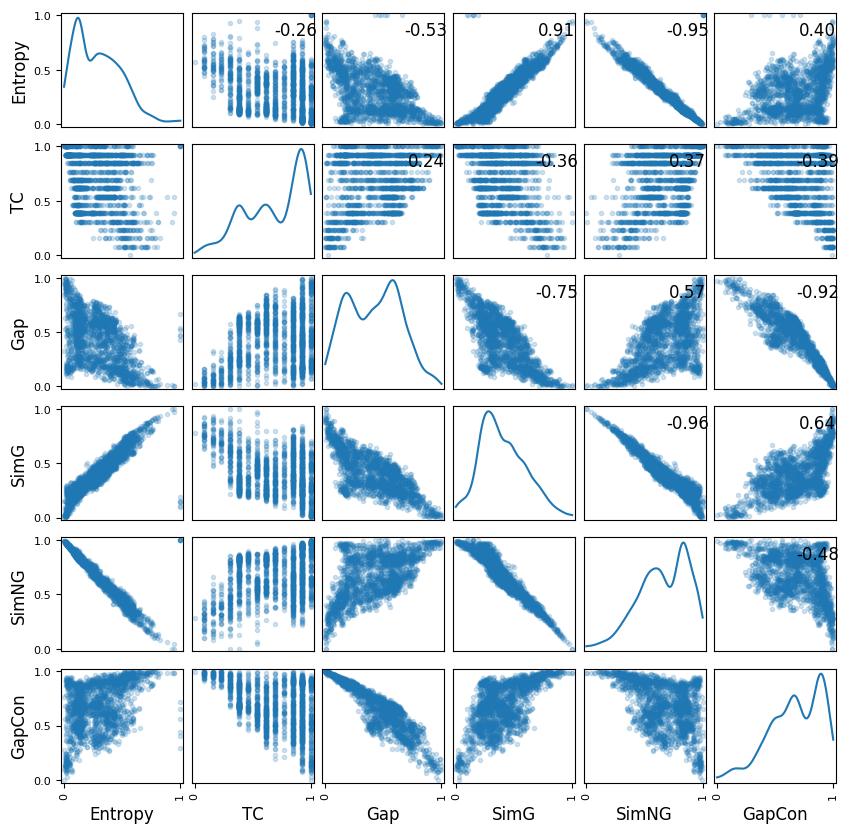
\includegraphics[width=\columnwidth]{Figure/6-obj-old/R0/fig/scatter_mattrix}
			\caption{R0}
			%\label{fig:con_pr09}
		\end{subfigure}	
		\begin{subfigure}{0.35\textwidth}
			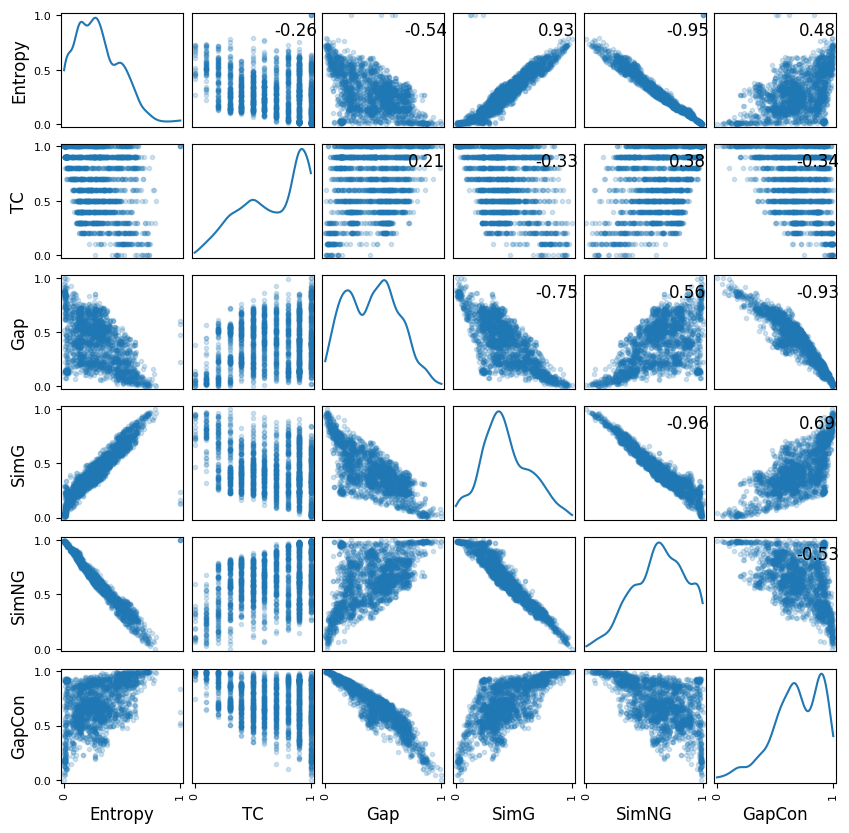
\includegraphics[width=\columnwidth]{Figure/6-obj-old/R4/fig/scatter_mattrix}
			\caption{R4}
			%\label{fig:con_pr09}
		\end{subfigure}
		\begin{subfigure}{0.35\textwidth}
			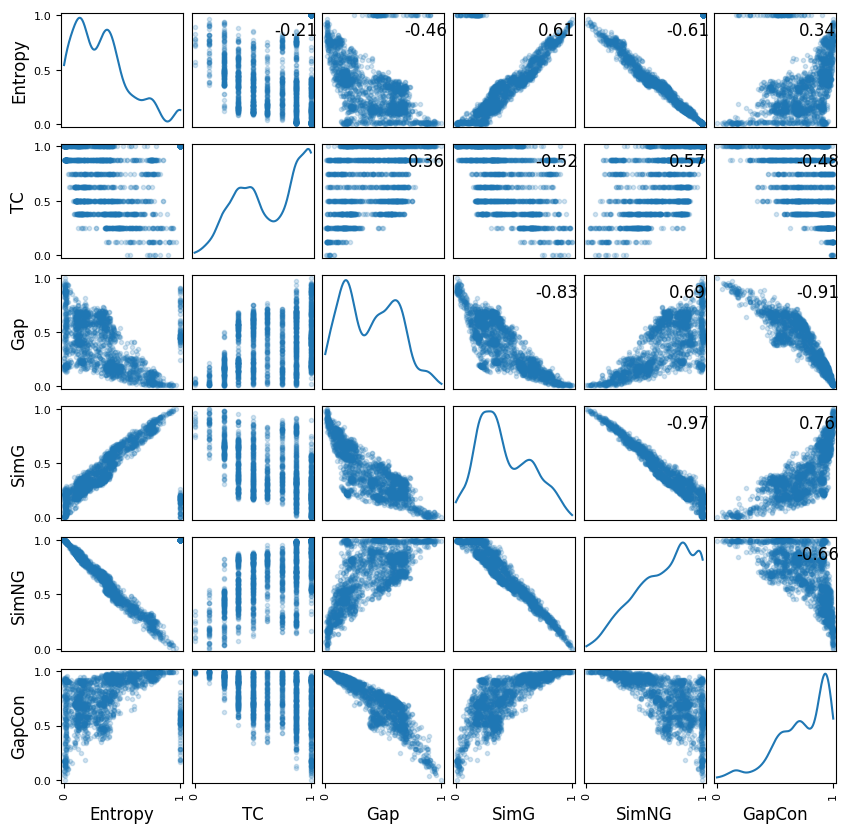
\includegraphics[width=\columnwidth]{Figure/6-obj-old/R9/fig/scatter_mattrix}
			\caption{R9}
			%\label{fig:con_pr09}
		\end{subfigure}
		\begin{subfigure}{0.35\textwidth}
			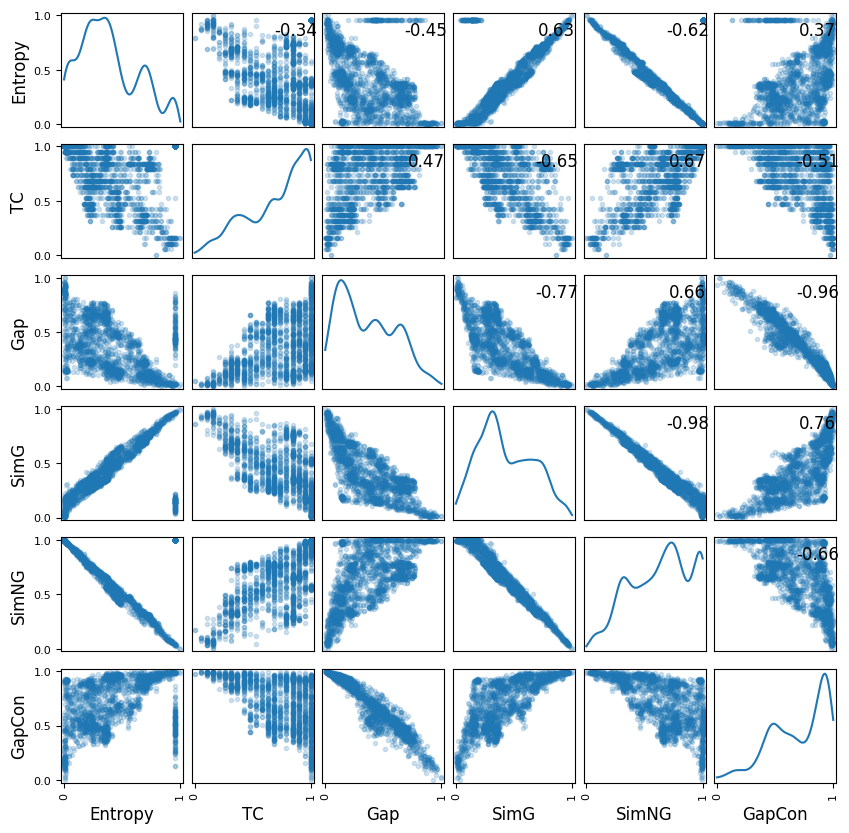
\includegraphics[width=\columnwidth]{Figure/6-obj-old/R14/fig/scatter_mattrix}
			\caption{R14}
			%\label{fig:con_pr09}
		\end{subfigure}
		\begin{subfigure}{0.35\textwidth}
			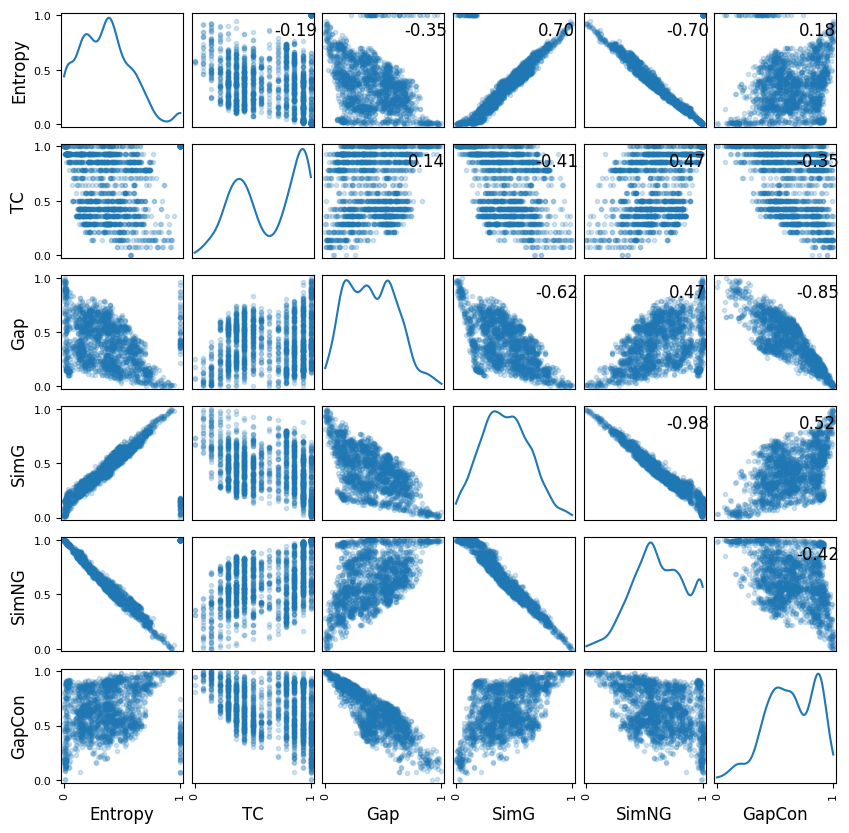
\includegraphics[width=\columnwidth]{Figure/6-obj-old/R19/fig/scatter_mattrix}
			\caption{R19}
			%\label{fig:con_pr09}
		\end{subfigure}
		\caption{Scatter-plot matrices depicting the pairwise relationship of all objective functions on five randomly selected replicates. We turn each objective function into minimization form and then normalize using min-max technique. In each matrix, the diagonal cells show the distribution of objective values (estimated using KDE) while the non-diagonal cells show the correlation between pairs of objective functions. Each upper-diagonal cell contains the value of correlation coefficient $r$ between the corresponding pair of objective functions.}
		\label{fig:new_nature_obj}
	\end{adjustwidth}
\end{figure*}
\begin{figure*}[!htbp]
	\centering
	\small
	\begin{adjustwidth}{-1cm}{-1cm}
		\begin{tabular}{l||C{0.24\textwidth}|C{0.24\textwidth}|C{0.24\textwidth}|C{0.24\textwidth} }
			& Entropy & GapCon & SimG & SimNG\\\hline\hline
			\rotatebox[origin=c]{-90}{R0} & 
			\raisebox{-.5\height}{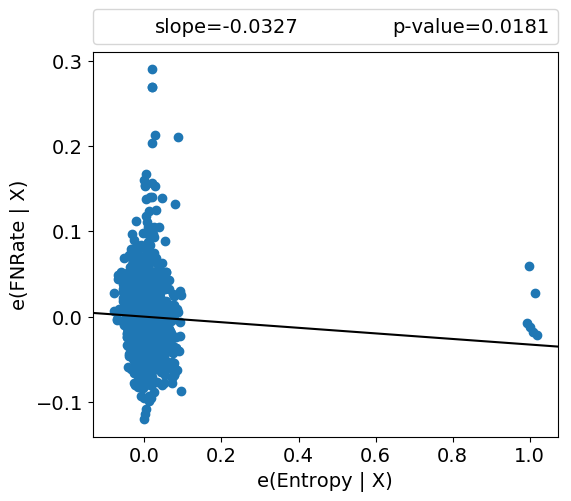
\includegraphics[width=0.25\textwidth]{Figure/6-obj-old/precomputedInit/R0/fig/Entropy_partial_regression}} &
			\raisebox{-.5\height}{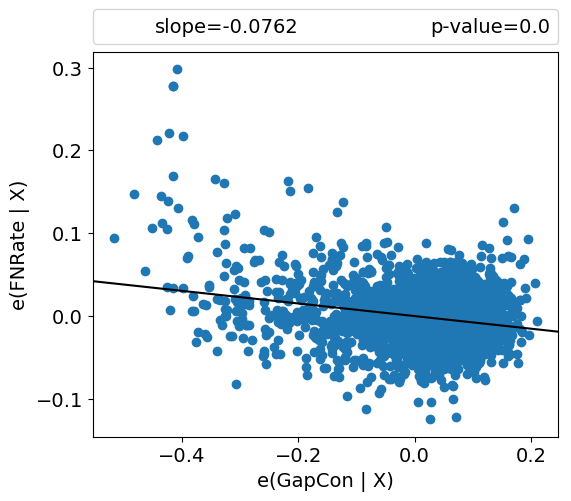
\includegraphics[width=0.25\textwidth]{Figure/6-obj-old/precomputedInit/R0/fig/GapCon_partial_regression}} & 
			\raisebox{-.5\height}{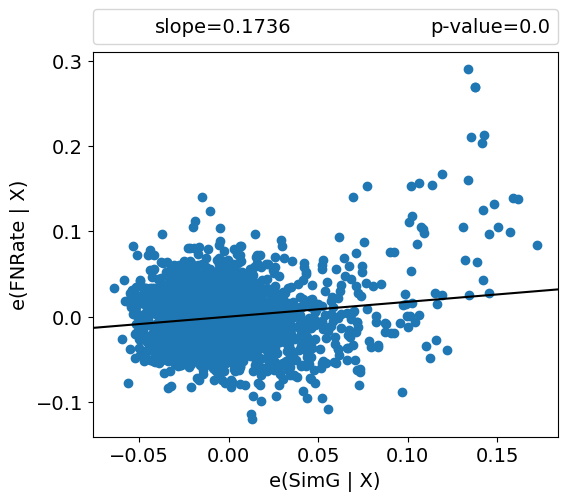
\includegraphics[width=0.25\textwidth]{Figure/6-obj-old/precomputedInit/R0/fig/SimG_partial_regression}} & 
			\raisebox{-.5\height}{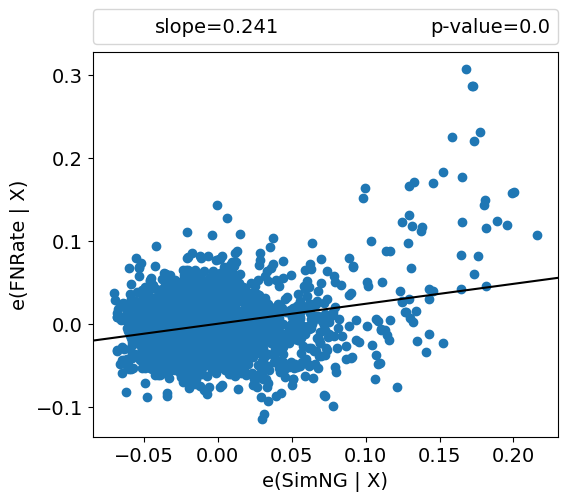
\includegraphics[width=0.25\textwidth]{Figure/6-obj-old/precomputedInit/R0/fig/SimNG_partial_regression}} 	
			\\\hline
			\rotatebox[origin=c]{-90}{R4} &
			\raisebox{-.5\height}{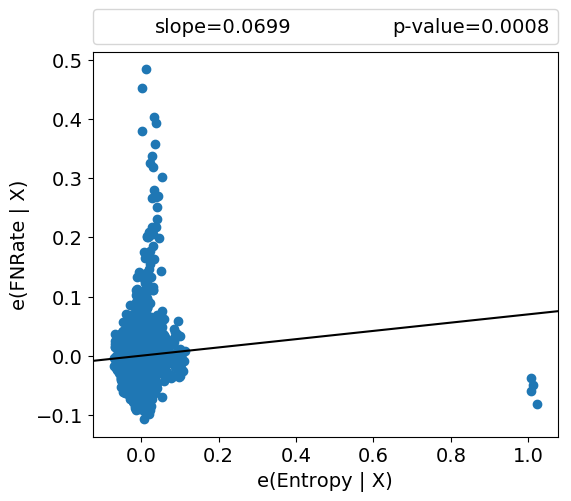
\includegraphics[width=0.25\textwidth]{Figure/6-obj-old/precomputedInit/R4/fig/Entropy_partial_regression}} &
			\raisebox{-.5\height}{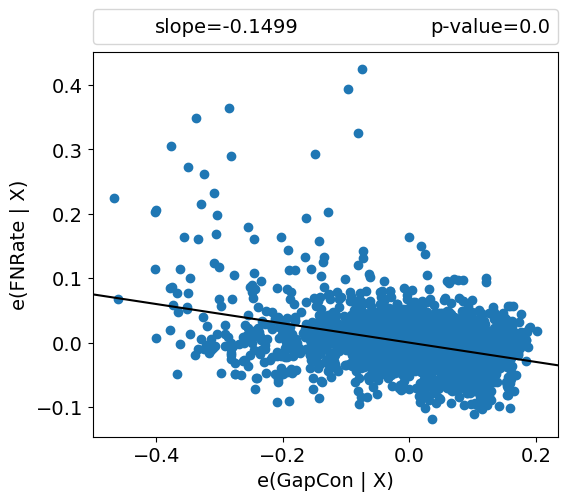
\includegraphics[width=0.25\textwidth]{Figure/6-obj-old/precomputedInit/R4/fig/GapCon_partial_regression}} & 
			\raisebox{-.5\height}{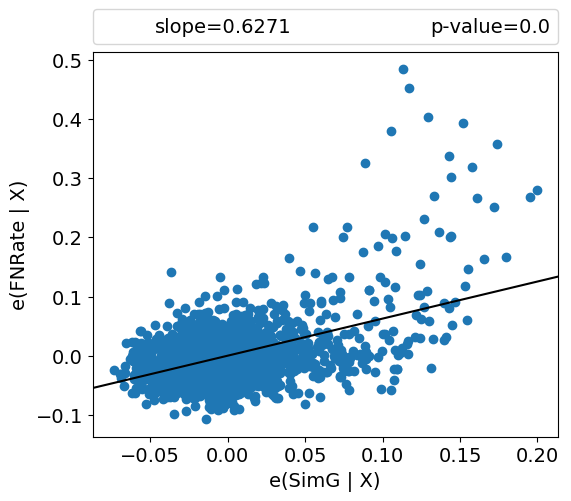
\includegraphics[width=0.25\textwidth]{Figure/6-obj-old/precomputedInit/R4/fig/SimG_partial_regression}} & 
			\raisebox{-.5\height}{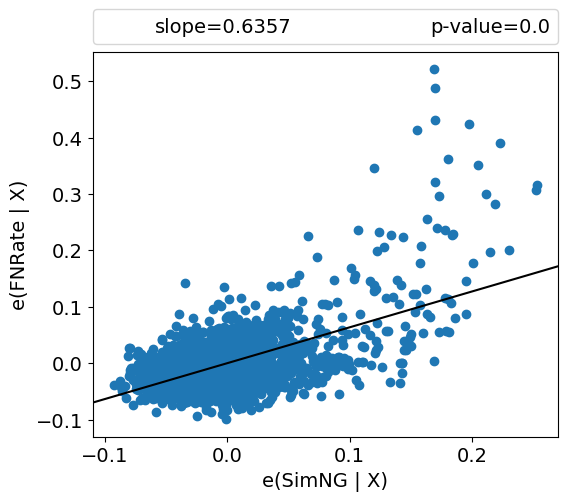
\includegraphics[width=0.25\textwidth]{Figure/6-obj-old/precomputedInit/R4/fig/SimNG_partial_regression}}
			\\\hline
			\rotatebox[origin=c]{-90}{R9} &
			\raisebox{-.5\height}{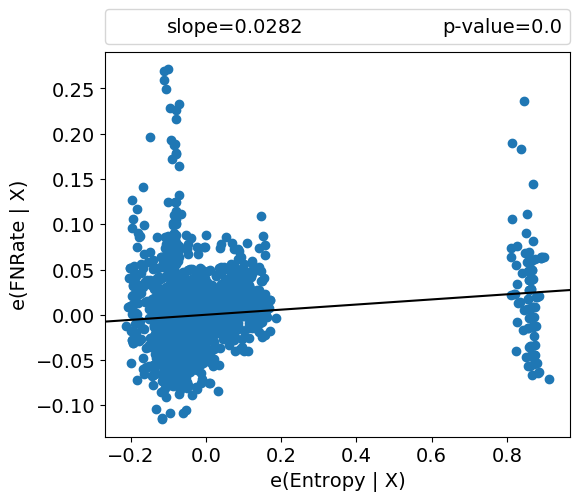
\includegraphics[width=0.25\textwidth]{Figure/6-obj-old/precomputedInit/R9/fig/Entropy_partial_regression}} &
			\raisebox{-.5\height}{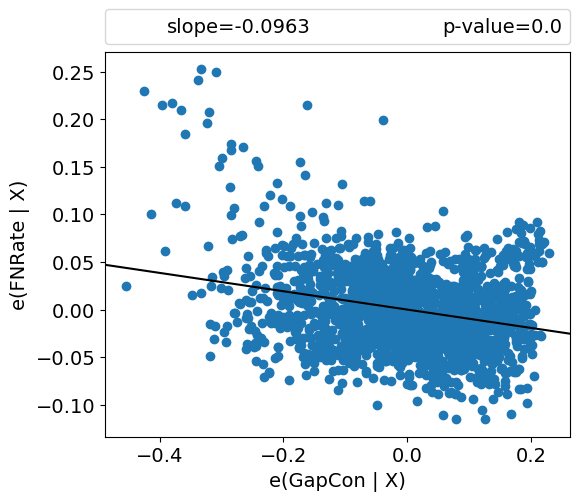
\includegraphics[width=0.25\textwidth]{Figure/6-obj-old/precomputedInit/R9/fig/GapCon_partial_regression}} & 
			\raisebox{-.5\height}{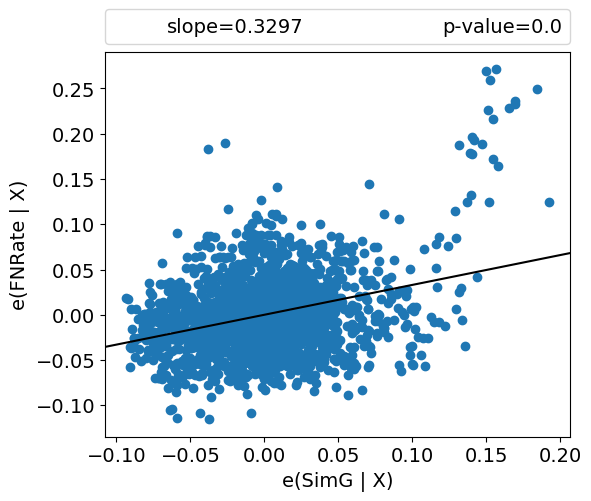
\includegraphics[width=0.25\textwidth]{Figure/6-obj-old/precomputedInit/R9/fig/SimG_partial_regression}} & 
			\raisebox{-.5\height}{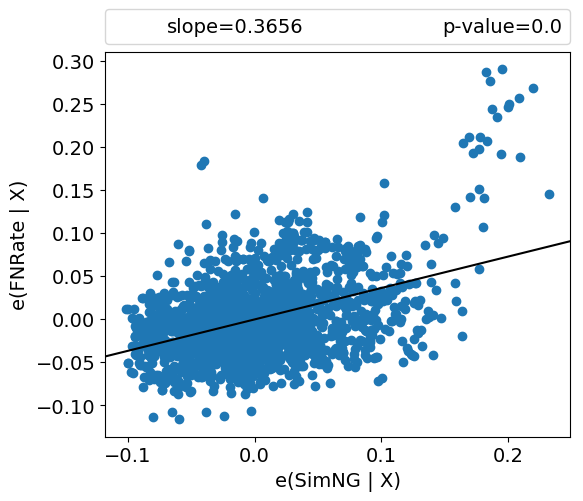
\includegraphics[width=0.25\textwidth]{Figure/6-obj-old/precomputedInit/R9/fig/SimNG_partial_regression}}
			\\\hline
			\rotatebox[origin=c]{-90}{R14} &
			\raisebox{-.5\height}{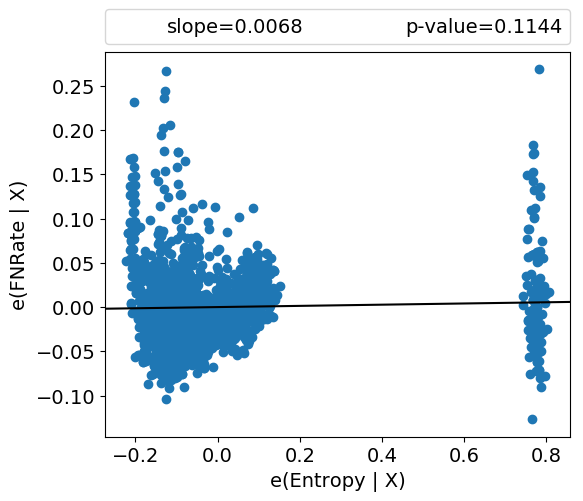
\includegraphics[width=0.25\textwidth]{Figure/6-obj-old/precomputedInit/R14/fig/Entropy_partial_regression}} &
			\raisebox{-.5\height}{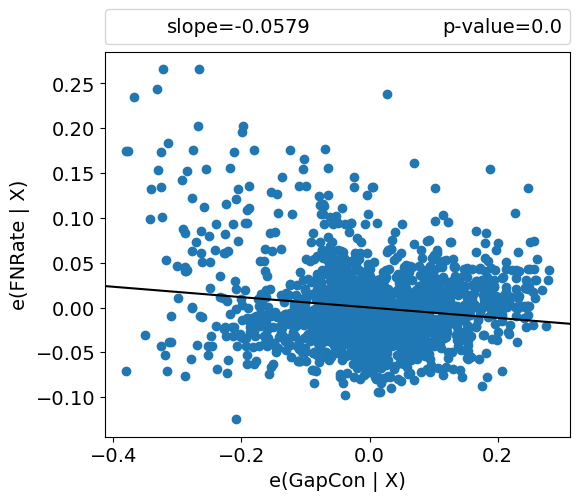
\includegraphics[width=0.25\textwidth]{Figure/6-obj-old/precomputedInit/R14/fig/GapCon_partial_regression}} & 
			\raisebox{-.5\height}{\includegraphics[width=0.25\textwidth]{Figure/6-obj-old/precomputedInit/R14/fig/SimG_partial_regression}} & 
			\raisebox{-.5\height}{\includegraphics[width=0.25\textwidth]{Figure/6-obj-old/precomputedInit/R14/fig/SimNG_partial_regression}}
			\\\hline
			\rotatebox[origin=c]{-90}{R19} &
			\raisebox{-.5\height}{\includegraphics[width=0.25\textwidth]{Figure/6-obj-old/precomputedInit/R19/fig/Entropy_partial_regression}} &
			\raisebox{-.5\height}{\includegraphics[width=0.25\textwidth]{Figure/6-obj-old/precomputedInit/R19/fig/GapCon_partial_regression}} & 
			\raisebox{-.5\height}{\includegraphics[width=0.25\textwidth]{Figure/6-obj-old/precomputedInit/R19/fig/SimG_partial_regression}} & 
			\raisebox{-.5\height}{\includegraphics[width=0.25\textwidth]{Figure/6-obj-old/precomputedInit/R19/fig/SimNG_partial_regression}}
			\\\hline
		\end{tabular}	
		\caption{Multiple linear regression model for identifying the association among FN rate and three objective functions (SimNG, GapCon and SimG/Entropy) fitted to five randomly selected replicates. There is one figure for each possible combination (replicate, objective function). Each partial regression plot shows the association between an objective function and FN rate while holding the remaining two objectives constant.  In a plot for an objective function $ OF $, the horizontal axis, $e(OF|X)$, denotes the residuals from regressing $OF$ against the remaining objective functions and the vertical axis, $e(FNRate|X)$, denotes the residuals from regressing FN rate against all the objective functions except $ OF $.}
		\label{fig:new_mul_lin_reg}
	\end{adjustwidth}
\end{figure*}
\subsubsection{Selection of a new formulation}
\label{sec:new_msa_formulation}
The results reported in the last subsection suggest that the objective functions that exhibit good association with FN rate should be more effective than the other objective functions for estimating phylogenetic trees. Based on this we make an attempt to form a new objective set as follows. We first propose four new objective functions that quantify different aspects of MSA: Entropy, SimG, SimNG and GapCon (the details are presented in Section~\ref{sec:formulation}). We combine these with TC and Gap and runNSGA-III to optimize the objective set \{Entropy, TC, Gap, SimG, SimNG, GapCon\} for 40 times to generate numerous diverse alignments. We used those to examine the association of our proposed objective functions with FN rate using multiple linear regression analysis. We depict the relationship between the relevant pairs of objective functions within the set in Figure~\ref{fig:new_nature_obj}. The key observations of this analysis are summarized as follows: 

\begin{itemize}
	\item Entropy has a strong correlation with SimG which is problematic for multiple regression analysis. So, we should not keep these two objectives at the same time in our regression model as well as in the multi-objective formulation.
	
	\item SimG and SimNG are in conflict with each other. So by optimizing them simulataneously, a multi-objective metaheuristic can generate large number of diverse alignments.
\end{itemize}

Now we express the relationship between FN rate and the proposed objective functions using the following model:
\begin{equation}
\small
\begin{split}
\text{FN rate} = \beta_0 + \beta_1 \times \text{SimNG}+ \beta_2 \times \text{GapCon} + \\
\beta_3 \times \text{SimG (or Entropy)} + \epsilon \label{eq:new_multi_lin_reg}
\end{split}
\end{equation}

We estimate the regression coefficients by fitting the above model to the solutions generated by optimizing the objective set \{Entropy, TC, Gap, SimG, SimNG, GapCon\}. We visualize the results using partial regression plots in Figure~\ref{fig:new_mul_lin_reg}. Here we see that, in each case, both SimG and SimNG exhibit positive correlation with FN rate. So we choose \{SimG, SimNG\} as our new objective set.

%\subsection{Results on biological rRNA datasets}

\begin{figure*}[!htbp]
	
	\begin{adjustwidth}{-1.5cm}{-1.5cm}
		\centering
		\begin{subfigure}{0.75\columnwidth}
			\includegraphics[width=\columnwidth]{Figure/summary/precomputedInit/avg_fnrate_density}
			\caption{Based on FN rate}
			%\label{fig:con_pr09}
		\end{subfigure}	
		\begin{subfigure}{0.75\columnwidth}
			\includegraphics[width=\columnwidth]{Figure/summary/precomputedInit/avg_tc_density}
			\caption{Based on TC score}
			%\label{fig:con_pr09}
		\end{subfigure}
		\begin{subfigure}{0.75\columnwidth}
			\includegraphics[width=\columnwidth]{Figure/summary/precomputedInit/avg_sp_density}
			\caption{Based on SP score}
			%\label{fig:con_pr09}
		\end{subfigure}
		\begin{subfigure}{0.75\columnwidth}
			\includegraphics[width=\columnwidth]{Figure/summary/precomputedInit/avg_objset_fnrate_rank}
			\caption{Based on FN rate}
			%\label{fig:con_pr09}
		\end{subfigure}	
		\begin{subfigure}{0.75\columnwidth}
			\includegraphics[width=\columnwidth]{Figure/summary/precomputedInit/avg_objset_tc_rank}
			\caption{Based on TC score}
			%\label{fig:con_pr09}
		\end{subfigure}
		\begin{subfigure}{0.75\columnwidth}
			\includegraphics[width=\columnwidth]{Figure/summary/precomputedInit/avg_objset_sp_rank}
			\caption{Based on SP score}
			%\label{fig:con_pr09}
		\end{subfigure}
	\caption{\underline{100-taxon simulated dataset:} Top panel (part (a) - (c)) illustrates how the 100 solutions provided by the multi-objective formulations perform with respect to each of the three metrics (FN rate, TC score, SP score) against the nine state-of-the-art tools. We average the scores of the multi-objective solutions in two steps. Since there are 100 solutions in each run, to make the average meaningful, we first sort the 100 solutions according to their scores. Now the scores of the best solutions along all the runs are averaged and taken as the best average score. The same applies for the second best ones and so on. Thus we get the 100 averaged scores for each replicate. Since all replicates actually represent one dataset, we again do a replicate wide averaging in the same way to get the scores of 100 solutions and then plotted them. Bottom panel (part (d) - (f)) illustrates how the score of the best solution (within 100 solutions), obtained by the multi-objective formulations, varies across 20 runs. To accomplish this, we collect the best scores (among 100 values) from 20 runs. Thus for each replicate, we get a set of 20 scores. We sort these 20 scores for each replicate and then perform replicate wide averaging ($n^{th}$ best scores from each replicate are averaged). Finally, we visualize the distribution of the averaged 20 scores using boxplot. In all figures, we depict the averaged scores of nine state-of-the-art tools over 10 replicates using dashed horizontal lines.}
	\label{fig:perf_100_taxon}
	\end{adjustwidth}
\end{figure*}


\subsection{Results on 100-taxon simulated dataset}
\label{sec:result_100_taxon}
Now we examine the performance of the two objective sets selected (in the previous sections), namely, \{Gap, SOP\} and \{SimG, SimNG\} on randomly chosen 10 replicates of 100-taxon simulated dataset against the state-of-the-art tools. Following the standard practice in the OR literature, we conduct 20 runs of NSGA-II for each possible combination (replicate, set of objective functions) due to its (NSGA-II) stochastic nature. Each run produces a set of 100 alignments that represent the trade-offs in satisfying all objectives under consideration. We first evaluate each alignment using the widely used metrics, namely, TC and SP score. Next, we estimate ML tree for each alignment and measure the FN rate of the resultant tree. We use the averaged TC score, SP score and FN rate over 10 replicates to evaluate the strength of each objective set from two perspectives in Figure~\ref{fig:perf_100_taxon}. %We now describe these results.


The top panel of Figure~\ref{fig:perf_100_taxon} (part (a) - (c)) illustrates how the 100 solutions provided by the multi-objective formulations perform with respect to each of the three metrics (FN rate, TC score, SP score) against the nine state-of-the-art tools. We average the scores of the multi-objective solutions in two steps. Since there are 100 solutions in each run, to make the average meaningful, we first sort the 100 solutions according to their scores. Now the scores of the best solutions along all the runs are averaged and taken as the best average score. The same applies for the second best ones and so on. Thus we get the 100 averaged scores for each replicate. Since all replicates actually represent one dataset, we again do a replicate wide averaging in the same way to get the scores of 100 solutions and then plotted them in part (a) to (c) of Figure~\ref{fig:perf_100_taxon}. For the state-of-the-art tools we only needed to average the deterministic score across 10 replicates. We depict these averaged scores using dashed horizontal lines. Moreover, as the 100 solutions are sort along the horizontal axis, it is easy to compare the performance.

In part (a) we notice that, \{Gap, SOP\} and \{SimG, SimNG\} achieve better FN rates than all state-of-the-art tools. We find PASTA to be the best among the nine tools, followed by T-Coffee. Among the solutions generated by \{SimG, SimNG\}, on average around, 15\% are better than PASTA and 50\% are better than T-Coffee. And as for \{Gap, SOP\}, on average around 10\% alignments are better than PASTA and 40\% are better than T-Coffee. However, these findings are in contrast with those based on the TC and SP scores (see part (b) and (c)). There we see that, the multi-objective formulations barely generate better solutions according to those measures than the best tool (i.e., PASTA).

Next we move to the bottom panel of Figure~\ref{fig:perf_100_taxon} (part (d) - (f)). Here we illustrate how the score of the best solution (within 100 solutions), obtained by the multi-objective formulations, varies across 20 runs. To do this, we collect the best scores (among 100 values) from 20 runs. Thus for each replicate, we get a set of 20 (best) scores. We sort these 20 scores for each replicate and then performed replicate wise averaging ($n^{th}$ best scores from each replicate are averaged) similar to what we did earlier. 
%This way, for 10 replicates we get 10 sets of FN rates containing 20 value. Then, we calculate one set from these 10 sets by averaging values at each position. 
Finally, we visualize the distribution of these averaged 20 scores using boxplots in part (d) to (f) of Figure~\ref{fig:perf_100_taxon}. Here we observe that, according to FN rate (part (d)), in case of both objective sets, almost all runs of the metaheuristics produce better solutions than the nine tools. 
%From the bottom end (the sample minimum), we see that both the multi-objective formulations can achieve around 30\% improvement compared to the best tool (PASTA). 
The box width (i.e., interquartile range) suggests that \{SimG, SimNG\} is slightly more consistent than \{Gap, SOP\}. But with respect to TC and SP score (part (e) and (f)), we notice that, the multi-objective formulations failed to outperform the best tools in significant portion of the cases. Clearly, this can be misleading in the context of phylogeny estimation. Therefore, the experimental results on 100-taxon simulated dataset clearly suggest that, the tools that perform the best based on widely used alignment quality scores are not necessarily the best with respect to phylogenetic tree estimation.
%So we conclude that, for 100-taxon simulated dataset \{SimG, SimNG\} performs better than \{Gap, SOP\}.

%\clearpage
\subsection{Results on biological rRNA datasets}
\begin{figure}[!htbp]
	\centering
	\begin{adjustwidth}{-0.2cm}{}
		\begin{subfigure}{0.5\columnwidth}
			\includegraphics[width=\columnwidth]{Figure/summary/precomputedInit/23S.E/fnrate_density_single_run}
			\caption{23S.E}
			%\label{fig:con_pr09}
		\end{subfigure}	
		\begin{subfigure}{0.5\columnwidth}
			\includegraphics[width=\columnwidth]{Figure/summary/precomputedInit/23S.E.aa_ag/fnrate_density_single_run}
			\caption{23S.E.aa\_ag}
			%\label{fig:con_pr09}
		\end{subfigure}
		\begin{subfigure}{0.5\columnwidth}
			\includegraphics[width=\columnwidth]{Figure/summary/precomputedInit/23S.E/objset_fnrate_rank}
			\caption{23S.E}
			%\label{fig:con_pr09}
		\end{subfigure}	
		\begin{subfigure}{0.5\columnwidth}
			\includegraphics[width=\columnwidth]{Figure/summary/precomputedInit/23S.E.aa_ag/objset_fnrate_rank}
			\caption{23S.E.aa\_ag}
			%\label{fig:con_pr09}
		\end{subfigure}
	\end{adjustwidth}
	\caption{\underline{Biological rRNA datasets:} Top panel (part (a), (b)) shows the averaged FN rate of 100 solutions over 10 runs. Since each run generates 100 solutions, we make the average meaningful by sorting the 100 FN rates per run. Then we average the best FN rates along all the runs. The same applies for the second best ones and so on. Bottom panel (part (c), (d)) shows the variation of the best FN rates across 10 runs using boxplots. In all figures, we show the performance of nine state-of-the-art tools using dashed horizontal lines.}
	\label{fig:fn_rate_bio}
\end{figure}

\begin{figure}[!htbp]
	\centering
	\begin{adjustwidth}{-0.2cm}{}
		\begin{subfigure}{0.5\columnwidth}
			\includegraphics[width=\columnwidth]{Figure/summary/precomputedInit/23S.E/tc_density_single_run}
			\caption{23S.E}
			%\label{fig:con_pr09}
		\end{subfigure}	
		\begin{subfigure}{0.5\columnwidth}
			\includegraphics[width=\columnwidth]{Figure/summary/precomputedInit/23S.E.aa_ag/tc_density_single_run}
			\caption{23S.E.aa\_ag}
			%\label{fig:con_pr09}
		\end{subfigure}
		\begin{subfigure}{0.5\columnwidth}
			\includegraphics[width=\columnwidth]{Figure/summary/precomputedInit/23S.E/objset_tc_rank}
			\caption{23S.E}
			%\label{fig:con_pr09}
		\end{subfigure}	
		\begin{subfigure}{0.5\columnwidth}
			\includegraphics[width=\columnwidth]{Figure/summary/precomputedInit/23S.E.aa_ag/objset_tc_rank}
			\caption{23S.E.aa\_ag}
			%\label{fig:con_pr09}
		\end{subfigure}
	\end{adjustwidth}
	\caption{\underline{Biological rRNA datasets:} Top panel (part (a), (b)) shows the TC score of 100  solutions averaged over 10 runs. At first, we sort the TC scores of each solution set. Then we average the TC scores at each sorted position of all the sets. Bottom panel (part (c), (d)) shows the distribution of the best TC scores collected from all runs. In each figure, The horizontal lines show the performance of the state-of-the-art tools.}
	\label{fig:tc_bio}
\end{figure}

\begin{figure}[!htbp]
	\centering
	\begin{adjustwidth}{-0.2cm}{}
		\begin{subfigure}{0.5\columnwidth}
			\includegraphics[width=\columnwidth]{Figure/summary/precomputedInit/23S.E/pairs_density_single_run}
			\caption{23S.E}
			%\label{fig:con_pr09}
		\end{subfigure}	
		\begin{subfigure}{0.5\columnwidth}
			\includegraphics[width=\columnwidth]{Figure/summary/precomputedInit/23S.E.aa_ag/pairs_density_single_run}
			\caption{23S.E.aa\_ag}
			%\label{fig:con_pr09}
		\end{subfigure}
		\begin{subfigure}{0.5\columnwidth}
			\includegraphics[width=\columnwidth]{Figure/summary/precomputedInit/23S.E/objset_pairs_rank}
			\caption{23S.E}
			%\label{fig:con_pr09}
		\end{subfigure}	
		\begin{subfigure}{0.5\columnwidth}
			\includegraphics[width=\columnwidth]{Figure/summary/precomputedInit/23S.E.aa_ag/objset_pairs_rank}
			\caption{23S.E.aa\_ag}
			%\label{fig:con_pr09}
		\end{subfigure}
	\end{adjustwidth}
	\caption{\underline{Biological rRNA datasets:} Top panel (part (a), (b)) shows the SP score of 100 solutions averaged over 10 runs. At first, we sort the SP scores of each solution set. Then we average the SP scores at each sorted position of all the sets. Bottom panel (part (c), (d)) shows the distribution of the best SP scores collected from all runs. In each figure, The horizontal lines show the performance of the state-of-the-art tools.}
	\label{fig:sp_bio}
\end{figure}

\begin{figure}[!htbp]
	\centering
	\begin{adjustwidth}{-0.2cm}{}
		\begin{subfigure}{0.5\columnwidth}
			\includegraphics[width=\columnwidth]{Figure/summary/precomputedInit/23S.E/fnrate_vs_tc}
			\caption{23S.E}
			%\label{fig:con_pr09}
		\end{subfigure}	
		\begin{subfigure}{0.5\columnwidth}
			\includegraphics[width=\columnwidth]{Figure/summary/precomputedInit/23S.E.aa_ag/fnrate_vs_tc}
			\caption{23S.E.aa\_ag}
			%\label{fig:con_pr09}
		\end{subfigure}
		\begin{subfigure}{0.5\columnwidth}
			\includegraphics[width=\columnwidth]{Figure/summary/precomputedInit/23S.E/fnrate_vs_sp}
			\caption{23S.E}
			%\label{fig:con_pr09}
		\end{subfigure}	
		\begin{subfigure}{0.5\columnwidth}
			\includegraphics[width=\columnwidth]{Figure/summary/precomputedInit/23S.E.aa_ag/fnrate_vs_sp}
			\caption{23S.E.aa\_ag}
			%\label{fig:con_pr09}
		\end{subfigure}
	\end{adjustwidth}
	\caption{\underline{Biological rRNA datasets:} Top panel (part (a), (b)) shows the relationship between FN rate and TC score for different alignments. And bottom panel (part (c), (d)) shows the relationship between FN rate and SP score. The horizontal lines mark the FN rates achieved by the state-of-the-art tools.}
	\label{fig:fnrate_vs_tc_bio}
\end{figure}
We conducted ten (instead of 20 as we did on 100-taxon dataset) runs of NSGA-II with our two selected objective sets (i.e., \{Gap ,SOP\} and \{SimG, SimNG\}) for two datasets, namely, 23S.E and 23S.E.aa\_ag. 

%In this section, we examine the resulting solution sets in terms of ML tree quality (i.e., FN rate) as well as alignment quality (i.e TC and SP score). We observed that MSA with better alignment quality (with respect to established scores) may not result into better phylogenetic tree.

%In the literature, we find the wide use of alignment quality to judge the effectiveness of a method. In this study, we would like to see whether the alignment quality goes in line with the tree quality.

We compare the performance of the multi-objective formulations with respect to FN rate against the nine state-of-the-art tools from two perspectives in Figure~\ref{fig:fn_rate_bio}. The top panel shows the averaged FN rate of 100 solutions over 10 runs. Since each run generates 100 solutions, we make the average meaningful by sorting the 100 FN rates per run . Then we average the best FN rates across all the runs. The same applies for the second best ones and so on. And the bottom panel summarizes the variation of the best FN rate (among 100 values) across 10 runs. For both of the datasets, FSA performs the best among the nine tools, followed by PRANK for 23.S.E and PASTA for 23S.E.aa\_ag. The two multi-objective formulations achieved better FN rates than FSA for 23S.E.aa\_ag (part (b) and (d)). Here, on average, \{Gap ,SOP\} generates around 10\% solutions that are better than FSA and 40\% solutions that are better than PASTA as shown in part (b). On the other hand, on average \{SimG, SimNG\} produces very few solutions that are better than FSA but around 40\% solutions that are better than PASTA. Part (d) shows that, \{Gap, SOP\} consistently outperforms the best tool (FSA) whereas \{SimG, SimNG\} outperforms FSA in nearly 40\% of the total runs. Now let us see the results for 23S.E, where both of the objective sets remain between the best (FSA) and second best (PRANK) tool. Both of them generates around 5\% solutions better than PRANK.
%and achieves around 30\% improvement compared to FSA.
%We visualize the distribution of the best FN rates collected from each run using boxplots in Figure~\ref{fig:fn_rate_bio}. In that figure, we also show the FN rates of 100 solutions. We see that for 23S.E.aa\_ag, both of the sets achieved FN rates better than the best tool FSA but \{Gap ,SOP\} is more consistent in generating good results. On the other hand, for 23S.E both the sets perform between the first and second best tool which is FSA and PRANK respectively. Here \{SimG, SimNG\} performs consistently better than the other.

We perform similar analysis based on the widely used two alignment quality measures, namely, TC score and SP score and report the results in Figure~\ref{fig:tc_bio} and \ref{fig:sp_bio} respectively. We notice that, according to these two popular measures, for both the datasets, the alignments generated by multi-objective formulations failed to beat the best performing tool, PASTA. The clear disagreement between FN rate and TC score (top panel) as well as between FN rate and SP score (bottom panel) has been illustrated in Figure~\ref{fig:fnrate_vs_tc_bio}. To summarize, from the analysis presented in Figure~\ref{fig:fnrate_vs_tc_bio}, we realize that the tools/approaches achieving better performance than our multi-objective formulations in terms of the popular measures, namely, TC score and SP score fail to achieve better FN rates than our multi-objective formulations. To elaborate, according to TC score, PASTA is the best performer among the nine tools, and our objective sets have generated several alignments having worse (lower) TC score than PASTA (and FSA). However those alignments can produce phylogenetic trees with better FN rates than those tools. Even from among the tools, there is disagreement between TC score and FN rate: PASTA is in fact behind FSA in terms of the latter. Similarly in the bottom panel of Figure~\ref{fig:fnrate_vs_tc_bio} which is dedicated to the comparison between FN rate and SP score, we find several alignments generated by the multi-objective formualtions that are worse than PASTA in terms of SP score, but, achieve better FN rates than that tool. 

%In Figure~\ref{fig:tc_bio}, we show similar results as above but based on the widely used alignment quality measure TC score. We notice that according to TC, the multi-objective formulations can hardly outperform the best tool PASTA for both of the datasets. However, interestingly our multi-objective formulations produces bettern phylogenetic trees. Therefore, the tool which produces better TC score does not necessarily produce better FN rate which is unexpected. We illustrate this disagreement between FN rate and TC score in the top panel of Figure~\ref{fig:fnrate_vs_tc_bio} where we plot the FN rate and TC score of the tools as well as best alignments generated by each objective set. We see that according to TC score, PASTA is the best tool while FSA performs the best based on FN rate. Moreover, our objective sets generated several alignments having worse (lower) TC score than PASTA and FSA. However, those alignments can produce phylogenetic trees with better FN rate than those tools.

%Finally, we perform similar analysis based on SP score as shown in Figure~\ref{fig:sp_bio}. Again, here we find similar disagreement between SP score and FN rate. For both the datasets, the alignments generated by the objective sets failed to beat the best tool PASTA according to SP score. We illustrate this phenomena in the bottom panel of Figure~\ref{fig:fnrate_vs_tc_bio}, where we find several alignments (generated by the multi-objective formulations) worse than PASTA (the best tool w.r.t. SP-score) achieve better FN rates than that tool.  


%\begin{comment}

%############################# RV11
\begin{figure*}[!htbp]
	\begin{adjustwidth}{-1cm}{-1cm}
	\centering
	\begin{subfigure}{0.22\textwidth}
		\includegraphics[width=\columnwidth]{Figure/summary/precomputedInit/Balibase/BB11005_fnrate_density_single_run}
		\caption{BB11005}
		%\label{fig:con_pr09}
	\end{subfigure}	
	\begin{subfigure}{0.22\textwidth}
		\includegraphics[width=\columnwidth]{Figure/summary/precomputedInit/Balibase/BB11018_fnrate_density_single_run}
		\caption{BB11018}
		%\label{fig:con_pr09}
	\end{subfigure}
	\begin{subfigure}{0.22\textwidth}
		\includegraphics[width=\columnwidth]{Figure/summary/precomputedInit/Balibase/BB11020_fnrate_density_single_run}
		\caption{BB11020}
		%\label{fig:con_pr09}
	\end{subfigure}
	\begin{subfigure}{0.22\textwidth}
		\includegraphics[width=\columnwidth]{Figure/summary/precomputedInit/Balibase/BB11033_fnrate_density_single_run}
		\caption{BB11033}
		%\label{fig:con_pr09}
	\end{subfigure}
%	\begin{subfigure}{0.22\textwidth}
%		\includegraphics[width=\columnwidth]{Figure/summary/precomputedInit/Balibase/BB11038_fnrate_density_single_run}
%		\caption{BB11038}
%		%\label{fig:con_pr09}
%	\end{subfigure}
	\begin{subfigure}{0.22\textwidth}
		\includegraphics[width=\columnwidth]{Figure/summary/precomputedInit/Balibase/BB11005_objset_fnrate_rank}
		\caption{BB11005}
		%\label{fig:con_pr09}
	\end{subfigure}	
	\begin{subfigure}{0.22\textwidth}
		\includegraphics[width=\columnwidth]{Figure/summary/precomputedInit/Balibase/BB11018_objset_fnrate_rank}
		\caption{BB11018}
		%\label{fig:con_pr09}
	\end{subfigure}
	\begin{subfigure}{0.22\textwidth}
		\includegraphics[width=\columnwidth]{Figure/summary/precomputedInit/Balibase/BB11020_objset_fnrate_rank}
		\caption{BB11020}
		%\label{fig:con_pr09}
	\end{subfigure}
	%		\begin{subfigure}{0.22\textwidth}
	%			\includegraphics[width=\columnwidth]{Figure/summary/precomputedInit/Balibase/BB11029_objset_fnrate_rank}
	%			\caption{BB11029}
	%			%\label{fig:con_pr09}
	%		\end{subfigure}
	\begin{subfigure}{0.22\textwidth}
		\includegraphics[width=\columnwidth]{Figure/summary/precomputedInit/Balibase/BB11033_objset_fnrate_rank}
		\caption{BB11033}
		%\label{fig:con_pr09}
	\end{subfigure}
	\caption{ \underline{RV11:} Top panel (part (a) - (d)) shows the FN rate of 100 solutions averaged over 20 runs. At first, we sort the FN rates of each solution set. Then we average the FN rates at each sorted position of all the sets. Bottom panel (part (e) - (h)) shows the distribution of the best FN rates collected from all runs. In each figure, the horizontal lines show the performance of the state-of-the-art tools.}
	%RV11: FN rate of 100 final solutions averaged over 20 runs. The FN rates are sorted for better visualization. The horizontal lines indicate FN rates achieved by the state-of-the-art tools. RV11: Distribution of the best FN rates collected from all runs. In each figure, the FN rate achieved by the state-of-the-art tools are shown as horizontal lines.
	\label{fig:rv11_fn_rate}
	\end{adjustwidth}
\end{figure*}


\begin{figure*}[!htbp]
	\begin{adjustwidth}{-1cm}{-1cm}
	\centering
		\begin{subfigure}{0.22\textwidth}
			\includegraphics[width=\columnwidth]{Figure/summary/precomputedInit/Balibase/BB11005_tc_density_single_run_2}
			\caption{BB11005}
			%\label{fig:con_pr09}
		\end{subfigure}	
		\begin{subfigure}{0.22\textwidth}
			\includegraphics[width=\columnwidth]{Figure/summary/precomputedInit/Balibase/BB11018_tc_density_single_run_2}
			\caption{BB11018}
			%\label{fig:con_pr09}
		\end{subfigure}
		\begin{subfigure}{0.22\textwidth}
			\includegraphics[width=\columnwidth]{Figure/summary/precomputedInit/Balibase/BB11020_tc_density_single_run_2}
			\caption{BB11020}
			%\label{fig:con_pr09}
		\end{subfigure}
%		\begin{subfigure}{0.22\textwidth}
%			\includegraphics[width=\columnwidth]{Figure/summary/precomputedInit/Balibase/BB11029_tc_density_single_run_2}
%			\caption{BB11029}
%			%\label{fig:con_pr09}
%		\end{subfigure}
		\begin{subfigure}{0.22\textwidth}
			\includegraphics[width=\columnwidth]{Figure/summary/precomputedInit/Balibase/BB11033_tc_density_single_run_2}
			\caption{BB11033}
			%\label{fig:con_pr09}
		\end{subfigure}
		\begin{subfigure}{0.22\textwidth}
			\includegraphics[width=\columnwidth]{Figure/summary/precomputedInit/Balibase/BB11005_objset_tc_rank_2}
			\caption{BB11005}
			%\label{fig:con_pr09}
		\end{subfigure}	
		\begin{subfigure}{0.22\textwidth}
			\includegraphics[width=\columnwidth]{Figure/summary/precomputedInit/Balibase/BB11018_objset_tc_rank_2}
			\caption{BB11018}
			%\label{fig:con_pr09}
		\end{subfigure}
		\begin{subfigure}{0.22\textwidth}
			\includegraphics[width=\columnwidth]{Figure/summary/precomputedInit/Balibase/BB11020_objset_tc_rank_2}
			\caption{BB11020}
			%\label{fig:con_pr09}
		\end{subfigure}
		%		\begin{subfigure}{0.22\textwidth}
		%			\includegraphics[width=\columnwidth]{Figure/summary/precomputedInit/Balibase/BB11029_objset_tc_rank_2}
		%			\caption{BB11029}
		%			%\label{fig:con_pr09}
		%		\end{subfigure}
		\begin{subfigure}{0.22\textwidth}
			\includegraphics[width=\columnwidth]{Figure/summary/precomputedInit/Balibase/BB11033_objset_tc_rank_2}
			\caption{BB11033}
			%\label{fig:con_pr09}
		\end{subfigure}
		\caption{\underline{RV11:} Top panel (part (a) - (d)) shows the TC score of 100 solutions averaged over 20 runs. At first, we sort the TC scores of each solution set. Then we average the TC scores at each sorted position of all the sets. Bottom panel (part (e) - (h)) shows the distribution of the best TC scores collected from all runs. In each figure, the horizontal lines show the performance of the state-of-the-art tools.}
		\label{fig:rv11_tc}
	\end{adjustwidth}
\end{figure*}


\begin{figure*}[!htbp]
	\begin{adjustwidth}{-1cm}{-1cm}
	\centering
		\begin{subfigure}{0.22\textwidth}
			\includegraphics[width=\columnwidth]{Figure/summary/precomputedInit/Balibase/BB11005_pairs_density_single_run_2}
			\caption{BB11005}
			%\label{fig:con_pr09}
		\end{subfigure}	
		\begin{subfigure}{0.22\textwidth}
			\includegraphics[width=\columnwidth]{Figure/summary/precomputedInit/Balibase/BB11018_pairs_density_single_run_2}
			\caption{BB11018}
			%\label{fig:con_pr09}
		\end{subfigure}
		\begin{subfigure}{0.22\textwidth}
			\includegraphics[width=\columnwidth]{Figure/summary/precomputedInit/Balibase/BB11020_pairs_density_single_run_2}
			\caption{BB11020}
			%\label{fig:con_pr09}
		\end{subfigure}
%		\begin{subfigure}{0.22\textwidth}
%			\includegraphics[width=\columnwidth]{Figure/summary/precomputedInit/Balibase/BB11029_pairs_density_single_run_2}
%			\caption{BB11029}
%			%\label{fig:con_pr09}
%		\end{subfigure}
		\begin{subfigure}{0.22\textwidth}
			\includegraphics[width=\columnwidth]{Figure/summary/precomputedInit/Balibase/BB11033_pairs_density_single_run_2}
			\caption{BB11033}
			%\label{fig:con_pr09}
		\end{subfigure}
		\begin{subfigure}{0.22\textwidth}
			\includegraphics[width=\columnwidth]{Figure/summary/precomputedInit/Balibase/BB11005_objset_pairs_rank_2}
			\caption{BB11005}
			%\label{fig:con_pr09}
		\end{subfigure}	
		\begin{subfigure}{0.22\textwidth}
			\includegraphics[width=\columnwidth]{Figure/summary/precomputedInit/Balibase/BB11018_objset_pairs_rank_2}
			\caption{BB11018}
			%\label{fig:con_pr09}
		\end{subfigure}
		\begin{subfigure}{0.22\textwidth}
			\includegraphics[width=\columnwidth]{Figure/summary/precomputedInit/Balibase/BB11020_objset_pairs_rank_2}
			\caption{BB11020}
			%\label{fig:con_pr09}
		\end{subfigure}
		%		\begin{subfigure}{0.22\textwidth}
		%			\includegraphics[width=\columnwidth]{Figure/summary/precomputedInit/Balibase/BB11029_objset_pairs_rank_2}
		%			\caption{BB11029}
		%			%\label{fig:con_pr09}
		%		\end{subfigure}
		\begin{subfigure}{0.22\textwidth}
			\includegraphics[width=\columnwidth]{Figure/summary/precomputedInit/Balibase/BB11033_objset_pairs_rank_2}
			\caption{BB11033}
			%\label{fig:con_pr09}
		\end{subfigure}
		\caption{\underline{RV11:} Top panel (part (a) - (d)) shows the SP score of 100 solutions averaged over 20 runs. At first, we sort the SP scores of each solution set. Then we average the SP scores at each sorted position of all the sets. Bottom panel (part (e) - (h)) shows the distribution of the best SP scores collected from all runs. In each figure, the horizontal lines show the performance of the state-of-the-art tools.}
		\label{fig:rv11_sp}
	\end{adjustwidth}
\end{figure*}

\begin{figure*}[!htbp]
	\begin{adjustwidth}{-1cm}{-1cm}
	\centering
		\begin{subfigure}{0.22\textwidth}
			\includegraphics[width=\columnwidth]{Figure/summary/precomputedInit/Balibase/BB11005_fnrate_vs_tc_2}
			\caption{BB11005}
			%\label{fig:con_pr09}
		\end{subfigure}	
		\begin{subfigure}{0.22\textwidth}
			\includegraphics[width=\columnwidth]{Figure/summary/precomputedInit/Balibase/BB11018_fnrate_vs_tc_2}
			\caption{BB11018}
			%\label{fig:con_pr09}
		\end{subfigure}
		\begin{subfigure}{0.22\textwidth}
			\includegraphics[width=\columnwidth]{Figure/summary/precomputedInit/Balibase/BB11020_fnrate_vs_tc_2}
			\caption{BB11020}
			%\label{fig:con_pr09}
		\end{subfigure}
		\begin{subfigure}{0.22\textwidth}
			\includegraphics[width=\columnwidth]{Figure/summary/precomputedInit/Balibase/BB11033_fnrate_vs_tc_2}
			\caption{BB11033}
			%\label{fig:con_pr09}
		\end{subfigure}	
		\begin{subfigure}{0.22\textwidth}
			\includegraphics[width=\columnwidth]{Figure/summary/precomputedInit/Balibase/BB11005_fnrate_vs_sp_2}
			\caption{BB11005}
			%\label{fig:con_pr09}
		\end{subfigure}	
		\begin{subfigure}{0.22\textwidth}
			\includegraphics[width=\columnwidth]{Figure/summary/precomputedInit/Balibase/BB11018_fnrate_vs_sp_2}
			\caption{BB11018}
			%\label{fig:con_pr09}
		\end{subfigure}
		\begin{subfigure}{0.22\textwidth}
			\includegraphics[width=\columnwidth]{Figure/summary/precomputedInit/Balibase/BB11020_fnrate_vs_sp_2}
			\caption{BB11020}
			%\label{fig:con_pr09}
		\end{subfigure}
		\begin{subfigure}{0.22\textwidth}
			\includegraphics[width=\columnwidth]{Figure/summary/precomputedInit/Balibase/BB11033_fnrate_vs_sp_2}
			\caption{BB11033}
			%\label{fig:con_pr09}
		\end{subfigure}	
		\caption{\underline{RV11:} Top panel (part (a) - (d)) shows the relationship between FN rate and TC score for different alignments. And bottom panel (part (e) - (h)) shows the relationship between FN rate and SP score. The horizontal lines mark the FN rates achieved by the state-of-the-art tools.}
		\label{fig:rv11_fnrate_vs_tc}
	\end{adjustwidth}
\end{figure*}
%############################# RV12
\begin{figure*}[!htbp]
	\centering
	\begin{adjustwidth}{-1cm}{-1cm}
		\begin{subfigure}{0.22\textwidth}
			\includegraphics[width=\columnwidth]{Figure/summary/precomputedInit/Balibase/BB12001_fnrate_density_single_run}
			\caption{BB12001}
			%\label{fig:con_pr09}
		\end{subfigure}	
		\begin{subfigure}{0.22\textwidth}
			\includegraphics[width=\columnwidth]{Figure/summary/precomputedInit/Balibase/BB12013_fnrate_density_single_run}
			\caption{BB12013}
			%\label{fig:con_pr09}
		\end{subfigure}
		\begin{subfigure}{0.22\textwidth}
			\includegraphics[width=\columnwidth]{Figure/summary/precomputedInit/Balibase/BB12022_fnrate_density_single_run}
			\caption{BB12022}
			%\label{fig:con_pr09}
		\end{subfigure}
		\begin{subfigure}{0.22\textwidth}
			\includegraphics[width=\columnwidth]{Figure/summary/precomputedInit/Balibase/BB12035_fnrate_density_single_run}
			\caption{BB12035}
			%\label{fig:con_pr09}
		\end{subfigure}
		\begin{subfigure}{0.22\textwidth}
			\includegraphics[width=\columnwidth]{Figure/summary/precomputedInit/Balibase/BB12044_fnrate_density_single_run}
			\caption{BB12044}
			%\label{fig:con_pr09}
		\end{subfigure}
		\begin{subfigure}{0.22\textwidth}
			\includegraphics[width=\columnwidth]{Figure/summary/precomputedInit/Balibase/BB12001_objset_fnrate_rank}
			\caption{BB12001}
			%\label{fig:con_pr09}
		\end{subfigure}	
		\begin{subfigure}{0.22\textwidth}
			\includegraphics[width=\columnwidth]{Figure/summary/precomputedInit/Balibase/BB12013_objset_fnrate_rank}
			\caption{BB12013}
			%\label{fig:con_pr09}
		\end{subfigure}
		\begin{subfigure}{0.22\textwidth}
			\includegraphics[width=\columnwidth]{Figure/summary/precomputedInit/Balibase/BB12022_objset_fnrate_rank}
			\caption{BB12022}
			%\label{fig:con_pr09}
		\end{subfigure}
		\begin{subfigure}{0.22\textwidth}
			\includegraphics[width=\columnwidth]{Figure/summary/precomputedInit/Balibase/BB12035_objset_fnrate_rank}
			\caption{BB12035}
			%\label{fig:con_pr09}
		\end{subfigure}
		\begin{subfigure}{0.22\textwidth}
			\includegraphics[width=\columnwidth]{Figure/summary/precomputedInit/Balibase/BB12044_objset_fnrate_rank}
			\caption{BB12044}
			%\label{fig:con_pr09}
		\end{subfigure}
		\caption{\underline{RV12:} Top panel (part (a) - (e)) shows the FN rate of 100 solutions averaged over 20 runs. At first, we sort the FN rates of each solution set. Then we average the FN rates at each sorted position of all the sets. Bottom panel (part (f) - (j)) shows the distribution of the best FN rates collected from all runs. In each figure, the horizontal lines show the performance of the state-of-the-art tools.}
		\label{fig:rv12_fn_rate}
	\end{adjustwidth}
\end{figure*}


\begin{figure*}[!htbp]
	\centering
	\begin{adjustwidth}{-1cm}{-1cm}
		\begin{subfigure}{0.22\textwidth}
			\includegraphics[width=\columnwidth]{Figure/summary/precomputedInit/Balibase/BB12001_tc_density_single_run_2}
			\caption{BB12001}
			%\label{fig:con_pr09}
		\end{subfigure}	
		\begin{subfigure}{0.22\textwidth}
			\includegraphics[width=\columnwidth]{Figure/summary/precomputedInit/Balibase/BB12013_tc_density_single_run_2}
			\caption{BB12013}
			%\label{fig:con_pr09}
		\end{subfigure}
		\begin{subfigure}{0.22\textwidth}
			\includegraphics[width=\columnwidth]{Figure/summary/precomputedInit/Balibase/BB12022_tc_density_single_run_2}
			\caption{BB12022}
			%\label{fig:con_pr09}
		\end{subfigure}
		\begin{subfigure}{0.22\textwidth}
			\includegraphics[width=\columnwidth]{Figure/summary/precomputedInit/Balibase/BB12035_tc_density_single_run_2}
			\caption{BB12035}
			%\label{fig:con_pr09}
		\end{subfigure}
		\begin{subfigure}{0.22\textwidth}
			\includegraphics[width=\columnwidth]{Figure/summary/precomputedInit/Balibase/BB12044_tc_density_single_run_2}
			\caption{BB12044}
			%\label{fig:con_pr09}
		\end{subfigure}
		%%%%%%%%%%%%%%
		\begin{subfigure}{0.22\textwidth}
			\includegraphics[width=\columnwidth]{Figure/summary/precomputedInit/Balibase/BB12001_objset_tc_rank_2}
			\caption{BB12001}
			%\label{fig:con_pr09}
		\end{subfigure}	
		\begin{subfigure}{0.22\textwidth}
			\includegraphics[width=\columnwidth]{Figure/summary/precomputedInit/Balibase/BB12013_objset_tc_rank_2}
			\caption{BB12013}
			%\label{fig:con_pr09}
		\end{subfigure}
		\begin{subfigure}{0.22\textwidth}
			\includegraphics[width=\columnwidth]{Figure/summary/precomputedInit/Balibase/BB12022_objset_tc_rank_2}
			\caption{BB12022}
			%\label{fig:con_pr09}
		\end{subfigure}
		\begin{subfigure}{0.22\textwidth}
			\includegraphics[width=\columnwidth]{Figure/summary/precomputedInit/Balibase/BB12035_objset_tc_rank_2}
			\caption{BB12035}
			%\label{fig:con_pr09}
		\end{subfigure}
		\begin{subfigure}{0.22\textwidth}
			\includegraphics[width=\columnwidth]{Figure/summary/precomputedInit/Balibase/BB12044_objset_tc_rank_2}
			\caption{BB12044}
			%\label{fig:con_pr09}
		\end{subfigure}
		\caption{\underline{RV12:} Top panel (part (a) - (e)) shows the TC score of 100 solutions averaged over 20 runs. At first, we sort the TC scores of each solution set. Then we average the TC scores at each sorted position of all the sets. Bottom panel (part (f) - (j)) shows the distribution of the best TC scores collected from all runs. In each figure, the horizontal lines show the performance of the state-of-the-art tools.}
		\label{fig:rv12_tc}
	\end{adjustwidth}
\end{figure*}


\begin{figure*}[!htbp]
	\centering
	\begin{adjustwidth}{-1cm}{-1cm}
		\begin{subfigure}{0.22\textwidth}
			\includegraphics[width=\columnwidth]{Figure/summary/precomputedInit/Balibase/BB12001_pairs_density_single_run_2}
			\caption{BB12001}
			%\label{fig:con_pr09}
		\end{subfigure}	
		\begin{subfigure}{0.22\textwidth}
			\includegraphics[width=\columnwidth]{Figure/summary/precomputedInit/Balibase/BB12013_pairs_density_single_run_2}
			\caption{BB12013}
			%\label{fig:con_pr09}
		\end{subfigure}
		\begin{subfigure}{0.22\textwidth}
			\includegraphics[width=\columnwidth]{Figure/summary/precomputedInit/Balibase/BB12022_pairs_density_single_run_2}
			\caption{BB12022}
			%\label{fig:con_pr09}
		\end{subfigure}
		\begin{subfigure}{0.22\textwidth}
			\includegraphics[width=\columnwidth]{Figure/summary/precomputedInit/Balibase/BB12035_pairs_density_single_run_2}
			\caption{BB12035}
			%\label{fig:con_pr09}
		\end{subfigure}
		\begin{subfigure}{0.22\textwidth}
			\includegraphics[width=\columnwidth]{Figure/summary/precomputedInit/Balibase/BB12044_pairs_density_single_run_2}
			\caption{BB12044}
			%\label{fig:con_pr09}
		\end{subfigure}
		\begin{subfigure}{0.22\textwidth}
			\includegraphics[width=\columnwidth]{Figure/summary/precomputedInit/Balibase/BB12001_objset_pairs_rank_2}
			\caption{BB12001}
			%\label{fig:con_pr09}
		\end{subfigure}	
		\begin{subfigure}{0.22\textwidth}
			\includegraphics[width=\columnwidth]{Figure/summary/precomputedInit/Balibase/BB12013_objset_pairs_rank_2}
			\caption{BB12013}
			%\label{fig:con_pr09}
		\end{subfigure}
		\begin{subfigure}{0.22\textwidth}
			\includegraphics[width=\columnwidth]{Figure/summary/precomputedInit/Balibase/BB12022_objset_pairs_rank_2}
			\caption{BB12022}
			%\label{fig:con_pr09}
		\end{subfigure}
		\begin{subfigure}{0.22\textwidth}
			\includegraphics[width=\columnwidth]{Figure/summary/precomputedInit/Balibase/BB12035_objset_pairs_rank_2}
			\caption{BB12035}
			%\label{fig:con_pr09}
		\end{subfigure}
		\begin{subfigure}{0.22\textwidth}
			\includegraphics[width=\columnwidth]{Figure/summary/precomputedInit/Balibase/BB12044_objset_pairs_rank_2}
			\caption{BB12044}
			%\label{fig:con_pr09}
		\end{subfigure}
		\caption{\underline{RV12:} Top panel (part (a) - (e)) shows the SP score of 100 solutions averaged over 20 runs. At first, we sort the SP scores of each solution set. Then we average the SP scores at each sorted position of all the sets. Bottom panel (part (f) - (j)) shows the distribution of the best SP scores collected from all runs. In each figure, the horizontal lines show the performance of the state-of-the-art tools.}
		\label{fig:rv12_sp}
	\end{adjustwidth}
\end{figure*}


\begin{figure*}[!htbp]
	\centering
	\begin{adjustwidth}{-1cm}{-1cm}
		\begin{subfigure}{0.22\textwidth}
			\includegraphics[width=\columnwidth]{Figure/summary/precomputedInit/Balibase/BB12001_fnrate_vs_tc_2}
			\caption{BB12001}
			%\label{fig:con_pr09}
		\end{subfigure}	
		\begin{subfigure}{0.22\textwidth}
			\includegraphics[width=\columnwidth]{Figure/summary/precomputedInit/Balibase/BB12013_fnrate_vs_tc_2}
			\caption{BB12013}
			%\label{fig:con_pr09}
		\end{subfigure}
		\begin{subfigure}{0.22\textwidth}
			\includegraphics[width=\columnwidth]{Figure/summary/precomputedInit/Balibase/BB12022_fnrate_vs_tc_2}
			\caption{BB12022}
			%\label{fig:con_pr09}
		\end{subfigure}
		\begin{subfigure}{0.22\textwidth}
			\includegraphics[width=\columnwidth]{Figure/summary/precomputedInit/Balibase/BB12035_fnrate_vs_tc_2}
			\caption{BB12035}
			%\label{fig:con_pr09}
		\end{subfigure}	
		\begin{subfigure}{0.22\textwidth}
			\includegraphics[width=\columnwidth]{Figure/summary/precomputedInit/Balibase/BB12044_fnrate_vs_tc_2}
			\caption{BB12044}
			%\label{fig:con_pr09}
		\end{subfigure}
		%%%%%%%%%
		\begin{subfigure}{0.22\textwidth}
			\includegraphics[width=\columnwidth]{Figure/summary/precomputedInit/Balibase/BB12001_fnrate_vs_sp_2}
			\caption{BB12001}
			%\label{fig:con_pr09}
		\end{subfigure}	
		\begin{subfigure}{0.22\textwidth}
			\includegraphics[width=\columnwidth]{Figure/summary/precomputedInit/Balibase/BB12013_fnrate_vs_sp_2}
			\caption{BB12013}
			%\label{fig:con_pr09}
		\end{subfigure}
		\begin{subfigure}{0.22\textwidth}
			\includegraphics[width=\columnwidth]{Figure/summary/precomputedInit/Balibase/BB12022_fnrate_vs_sp_2}
			\caption{BB12022}
			%\label{fig:con_pr09}
		\end{subfigure}
		\begin{subfigure}{0.22\textwidth}
			\includegraphics[width=\columnwidth]{Figure/summary/precomputedInit/Balibase/BB12035_fnrate_vs_sp_2}
			\caption{BB12035}
			%\label{fig:con_pr09}
		\end{subfigure}	
		\begin{subfigure}{0.22\textwidth}
			\includegraphics[width=\columnwidth]{Figure/summary/precomputedInit/Balibase/BB12044_fnrate_vs_sp_2}
			\caption{BB12044}
			%\label{fig:con_pr09}
		\end{subfigure}
		\caption{\underline{RV12}: Top panel (part (a) - (e)) shows the relationship between FN rate and TC score for different alignments. And bottom panel (part (f) - (j)) shows the relationship between FN rate and SP score. The horizontal lines mark the FN rates achieved by the state-of-the-art tools.}
		\label{fig:rv12_fnrate_vs_tc}
	\end{adjustwidth}
\end{figure*}

%\end{comment}
\subsection{Results on BAliBASE datasets}
For each of the selected BAliBASE datasets under six groups (RV11, RV12, RV20, RV30, RV40 and RV50), we conducted 20 independent runs of NSGA-II considering its stochastic nature according to the standard practice of OR literature. Once again we analyze the generated solutions based on the quality of alignments and resultant trees. We witnessed that the alignments that are better according to widely accepted alignment scores, not necessarily generate better phylogenetic trees.
%As the results for all the groups are very similar and consistent with our previous findings, in this section we present the results for RV11 and RV12. The results for the other groups can be found in the supplementary material.

Let us observe the results for four datasets under group RV11. According to FN rate (Figure \ref{fig:rv11_fn_rate}), at least one of the two objective sets generates better or equivalent solutions than the best tool throughout all the instances. For BB11020, \{SimG, SimNG\} can achieve 12\% FN rate as opposed to 50\% FN rate attained by the best tool which is a huge improvement. Considering TC score (Figure \ref{fig:rv11_tc}), the two objective sets can outperform all the tools only for BB11020 which is contrary to the findings based on FN rate. So again we see the disagreement between FN rate and TC score which we examine graphically in the top panel of Figure~\ref{fig:rv11_fnrate_vs_tc}. If we observe the results based on SP score (Figure \ref{fig:rv11_sp}), we get similar disagreement between FN rate and SP score which is illustrated in the bottom panel of Figure~\ref{fig:rv11_fnrate_vs_tc}. These figures provide evidence that a solution with the best TC and/or SP score may not give the best FN rate.
%. These are relatively small datasets with 8-14 taxa. And each of the two objective set performs better than the other for two cases. 

Next, we discuss our findings for the five datasets under group RV12. Here According to FN rate (Figure \ref{fig:rv12_fn_rate}), the multi-objective formulations outperform all the state-of-the-art tools for BB12013 and BB12035. In case of BB12035, \{SimG, SimNG\} shows remarkable improvement in FN rate (0\% vs 20\%) compared to the best tool. For the remaining datasets (BB12001 and BB12022), the multi-objective formulations perform as good as the best tool. On all the datasets, the two objective sets generate several solutions that are equivalent or better than that of the best tool.
%the two objective sets generate several solutions that are similar to or better than the best tool on all the datasets. And the set \{SimG, SimNG\} performs better than \{Gap, SOP\} except for BB12044. 
However, as observed in previous datasets, we see contrasting results with respect to TC and SP score (Figure \ref{fig:rv12_tc},\ref{fig:rv12_sp}). Here we find only a few cases where the two objective sets can outperform the best tool. We closely analyze this issue in Figure~\ref{fig:rv12_fnrate_vs_tc} where we find that there are several solutions that achieve better FN rates in spite of their poor alignment quality (TC and SP score).

%Also, SP score (Figure \ref{fig:rv12_sp}) gives similar message more or less.

For the remaining groups (RV20, RV30, RV40 and RV50), our obtained results are very similar and consistent with our previous findings. For the sake of brevity, we present those results in Section~\ref{sec:result_balibase} of the supplementary material.


Now we confirm the significance of the improvement achieved by the multi-objective formulations in terms of FN rate over nine MSA tools on 27 BAliBASE datasets by applying an appropriate statistical test. We form paired data by picking the FN rate achieved by each (MSA method, dataset) pair. For the metaheuristics, we take the average of the 20 best FN rates from 20 independent runs considering its stochastic nature. As our data do not satisfy the condition of normality and homoscedasticity~\citep{sheskin2003handbook}, we choose a series of  nonparametric tests following the recommendation of~\cite{derrac2011practical}. 
At first, we simultaneously compare all the methods using the Friedman test~\citep{friedman1937use} which gives the relative ranking (lower is better) of all the methods and strongly suggests the existence of significant differences among the methods considered (as $p$-value is 0). Table~\ref{tab:friedman_rank} shows these results. Here we see that the multi-objective formulations achieve the top two positions. 
Next, we complement the Friedman test by following Holm's post-hoc procedure~\citep{holm1979simple} to contrast the difference between the multi-objective formulations and each of the nine tools. Table~\ref{tab:holm_test} summarizes the results. Here, each cell shows the adjusted $p$-value which indicates the significance of difference in performance (based on FN rate) between two methods. We notice that all the $p$-values are very close to 0 and the values for \{SimG, SimNG\} are lower than \{Gap, SOP\}. So we can state with high confidence that, the multi-objective formulations achieve statistically significant improvement over the nine MSA tools.



% Table generated by Excel2LaTeX from sheet 'Sheet5'
\begin{table}[htbp]
	\small
	\centering
	\caption{The Average Friedman's ranking (lower is better) achieved by the MSA methods over 27 BAliBASE datasets. We performed the Friedman test based on FN rate achieved by the tools. For our metaheuristics based multi-objective formulations, we consider the average of the 20 best FN rates obtained from 20 runs. We also show the computed statistics and corresponding $ p $-value. }
	\begin{tabular}{|l|r|}
		\hline
		\multicolumn{1}{|c|}{Method} & \multicolumn{1}{c|}{Rank} \\
		\hline
		NSGA-II$_{\text{\{SimG, SimNG\}}}$ & 2.2037 \\
		\hline
		NSGA-II$_{\text{\{Gap, SOP\}}}$ & 2.8704 \\
		\hline
		ProbCons & 5.7963 \\
		\hline
		Clustal $\Omega$ & 6.2963 \\
		\hline
		MAFFT & 6.4074 \\
		\hline
		Kalign & 6.7037 \\
		\hline
		PASTA & 6.8148 \\
		\hline
		FSA   & 6.9444 \\
		\hline
		MUSCLE & 7.1482 \\
		\hline
		Clustal W & 7.3519 \\
		\hline
		RetAlign & 7.4630 \\
		\hline
		\hline
		\multicolumn{1}{|c|}{Statistic} & 10.5911 \\
		\hline
		\multicolumn{1}{|c|}{$ p $-value} & 0.0000 \\
		\hline
	\end{tabular}%
	\label{tab:friedman_rank}%
\end{table}%


% Table generated by Excel2LaTeX from sheet 'Sheet5'
\begin{table*}[htbp]
	\small
	\centering
	\begin{adjustwidth}{-2cm}{-2cm}
	\caption{Comparison between the metaheuristics and the MSA tool using the Holm's post-hoc procedures (as a complement of the Friedman test) over 27 BAliBASE datasets. Each entry shows the adjusted $p$-value which indicates the significance of difference in performance (based on FN rate) between two methods.} %We used the best ranked method (i.e. NSGA-II$_{\text{\{SimG, SimNG\}}}$) as the control method
	\begin{tabular}{|l|r|r|r|r|r|r|r|r|r|}
		\hline
		& RetAlign & Clustal W & MUSCLE & FSA   & PASTA & Kalign & MAFFT & Clustal $\Omega$ & ProbCons  \\
		\hline
		NSGA-II$_{\text{\{SimG, SimNG\}}}$& 0.00000 & 0.00000 & 0.00000 & 0.00000 & 0.00000 & 0.00000 & 0.00001 & 0.00002 & 0.00014  \\
		\hline
		NSGA-II$_{\text{\{Gap, SOP\}}}$ & 0.00000 & 0.00001 & 0.00002 & 0.00004 & 0.00007 & 0.00011 & 0.00036 & 0.00044 & 0.00238  \\
		\hline
	\end{tabular}%
	\label{tab:holm_test}%
	\end{adjustwidth}
\end{table*}%



\begin{comment}

Thirdly, the results for the five datasets under group RV20 are presented here.  Here According to FN rate (Figure \ref{fig:rv20_density_fn_rate} - \ref{fig:rv20_boxplot_fnrate}), the two objective sets generate several solutions that are similar to or better than the best tool on all the datasets. And the set \{SimG, SimNG\} performs better than \{Gap, SOP\} except for BB20022 and BB20033. However, we see somewhat opposite results . Again we find that the two objective sets struggle to beat the best tool considering TC score (Figure \ref{fig:rv20_density_tc} - \ref{fig:rv20_boxplot_tc}). Figure~\ref{fig:rv20_fnrate_vs_tc} shows the anomaly between TC score and FN rate. Also, SP score (Figure \ref{fig:rv20_density_pairs} - \ref{fig:rv20_boxplot_pairs}) gives almost similar message.

Fourthly, we look into group RV30 with four datasets. Here we find that two the objective sets produces better FN rate than the best tools (Figure \ref{fig:rv30_density_fn_rate} - \ref{fig:rv30_boxplot_fnrate}). And each of the two objective set performs better than the other for two cases. Also we find the anomaly between FN rate and TC score as well as SP score (Figure \ref{fig:rv30_density_tc} - \ref{fig:rv30_fnrate_vs_tc}).

Fifthly, we present our findings for the five datasets under group RV40. Here we see that, for all the datasets either of the two objective sets produces the best FN rate (Figure \ref{fig:rv40_density_fn_rate} - \ref{fig:rv40_boxplot_fnrate}). For some datasets \{SimG, SimNG\} performs better, while for the other datasets \{Gap, SOP\} performs better. Considering TC and SP score, we see similar disagreement with FN rate (Figure \ref{fig:rv40_density_tc} - \ref{fig:rv40_fnrate_vs_tc}).

Lastly, we look at the results for the four datasets of group RV50 (Figure \ref{fig:rv50_density_fn_rate} - \ref{fig:rv50_fnrate_vs_tc}).  These results are similar to the previous groups.
\end{comment}


\begin{comment}
\begin{figure}[!htbp]
\centering
\begin{adjustwidth}{-0.2cm}{}
\begin{subfigure}{0.5\columnwidth}
\includegraphics[width=\columnwidth]{Figure/summary/precomputedInit/23S.E/objset_fnrate_rank}
\caption{23S.E}
%\label{fig:con_pr09}
\end{subfigure}	
\begin{subfigure}{0.5\columnwidth}
\includegraphics[width=\columnwidth]{Figure/summary/precomputedInit/23S.E.aa_ag/objset_fnrate_rank}
\caption{23S.E.aa\_ag}
%\label{fig:con_pr09}
\end{subfigure}
\end{adjustwidth}
\caption{Biological rRNA datasets: Distribution of the best FN rates collected from all runs.  The horizontal lines show the performance of the state-of-the-art tools.}
\label{fig:best_fn_rate_bio}
\end{figure}
\begin{figure}[!htbp]
\centering
\includegraphics[width=0.7\columnwidth]{Figure/summary/precomputedInit/bar_objset_good_msa_count}
\caption{Comparison among objective sets based on total number of generated alignments that results better or equal FN rate than all the state-of-the-art tools.}
\label{fig:rank_good_msa_count}
\end{figure}
\begin{figure*}[!htbp]
\centering
\begin{subfigure}{0.26\textwidth}
\includegraphics[width=\columnwidth]{Figure/NumGaps_SOP/precomputedInit/R0/fnrate_density_single_run}
\caption{R0}
%\label{fig:con_pr09}
\end{subfigure}	
\begin{subfigure}{0.26\textwidth}
\includegraphics[width=\columnwidth]{Figure/NumGaps_SOP/precomputedInit/R4/fnrate_density_single_run}
\caption{R4}
%\label{fig:con_pr09}
\end{subfigure}
\begin{subfigure}{0.26\textwidth}
\includegraphics[width=\columnwidth]{Figure/NumGaps_SOP/precomputedInit/R9/fnrate_density_single_run}
\caption{R9}
%\label{fig:con_pr09}
\end{subfigure}
\begin{subfigure}{0.26\textwidth}
\includegraphics[width=\columnwidth]{Figure/NumGaps_SOP/precomputedInit/R14/fnrate_density_single_run}
\caption{R14}
%\label{fig:con_pr09}
\end{subfigure}
\begin{subfigure}{0.26\textwidth}
\includegraphics[width=\columnwidth]{Figure/NumGaps_SOP/precomputedInit/R19/fnrate_density_single_run}
\caption{R19}
%\label{fig:con_pr09}
\end{subfigure}
\caption{Density of FN rate across the members of a pareto front. In each figure, the FN rate achieved by the state-of-the-art tools are shown as vertical lines.}
\label{fig:density_fn_rate}
\end{figure*}

\begin{figure}[!htbp]
\centering
\includegraphics[width=0.6\columnwidth]{Figure/NumGaps_SOP_TC_wSOP/precomputedInit/fig/objset_rsquared_rank}
\caption{Comparison of objective sets based on how close they can explain FN rate. Here we keep the results for the set \{TC, Gap, SOP\} as the baseline.}
\label{fig:rank_adjusted_r}
\end{figure}

\begin{figure*}[!h]
\centering
\small
\begin{adjustwidth}{-1cm}{}
\begin{tabular}{l||C{0.24\textwidth}|C{0.24\textwidth}|C{0.24\textwidth}|C{0.24\textwidth} }
& TC & Gap & SOP & wSOP\\\hline\hline
\rotatebox[origin=c]{-90}{R0} & 
\raisebox{-.5\height}{\includegraphics[width=0.25\textwidth]{Figure/NumGaps_SOP_TC_wSOP/precomputedInit/R0/fig/tc_good_msa_hist}} &
\raisebox{-.5\height}{\includegraphics[width=0.25\textwidth]{Figure/NumGaps_SOP_TC_wSOP/precomputedInit/R0/fig/gap_good_msa_hist}} & 
\raisebox{-.5\height}{\includegraphics[width=0.25\textwidth]{Figure/NumGaps_SOP_TC_wSOP/precomputedInit/R0/fig/sop_good_msa_hist}} & 
\raisebox{-.5\height}{\includegraphics[width=0.25\textwidth]{Figure/NumGaps_SOP_TC_wSOP/precomputedInit/R0/fig/wsop_good_msa_hist}} 	
\\\hline
\rotatebox[origin=c]{-90}{R4} &
\raisebox{-.5\height}{\includegraphics[width=0.25\textwidth]{Figure/NumGaps_SOP_TC_wSOP/precomputedInit/R4/fig/tc_good_msa_hist}} &
\raisebox{-.5\height}{\includegraphics[width=0.25\textwidth]{Figure/NumGaps_SOP_TC_wSOP/precomputedInit/R4/fig/gap_good_msa_hist}} & 
\raisebox{-.5\height}{\includegraphics[width=0.25\textwidth]{Figure/NumGaps_SOP_TC_wSOP/precomputedInit/R4/fig/sop_good_msa_hist}} & 
\raisebox{-.5\height}{\includegraphics[width=0.25\textwidth]{Figure/NumGaps_SOP_TC_wSOP/precomputedInit/R4/fig/wsop_good_msa_hist}}
\\\hline
\rotatebox[origin=c]{-90}{R9} &
\raisebox{-.5\height}{\includegraphics[width=0.25\textwidth]{Figure/NumGaps_SOP_TC_wSOP/precomputedInit/R9/fig/tc_good_msa_hist}} &
\raisebox{-.5\height}{\includegraphics[width=0.25\textwidth]{Figure/NumGaps_SOP_TC_wSOP/precomputedInit/R9/fig/gap_good_msa_hist}} & 
\raisebox{-.5\height}{\includegraphics[width=0.25\textwidth]{Figure/NumGaps_SOP_TC_wSOP/precomputedInit/R9/fig/sop_good_msa_hist}} & 
\raisebox{-.5\height}{\includegraphics[width=0.25\textwidth]{Figure/NumGaps_SOP_TC_wSOP/precomputedInit/R9/fig/wsop_good_msa_hist}}
\\\hline
\rotatebox[origin=c]{-90}{R14} &
\raisebox{-.5\height}{\includegraphics[width=0.25\textwidth]{Figure/NumGaps_SOP_TC_wSOP/precomputedInit/R14/fig/tc_good_msa_hist}} &
\raisebox{-.5\height}{\includegraphics[width=0.25\textwidth]{Figure/NumGaps_SOP_TC_wSOP/precomputedInit/R14/fig/gap_good_msa_hist}} & 
\raisebox{-.5\height}{\includegraphics[width=0.25\textwidth]{Figure/NumGaps_SOP_TC_wSOP/precomputedInit/R14/fig/sop_good_msa_hist}} & 
\raisebox{-.5\height}{\includegraphics[width=0.25\textwidth]{Figure/NumGaps_SOP_TC_wSOP/precomputedInit/R14/fig/wsop_good_msa_hist}}
\\\hline
\rotatebox[origin=c]{-90}{R19} &
\raisebox{-.5\height}{\includegraphics[width=0.25\textwidth]{Figure/NumGaps_SOP_TC_wSOP/precomputedInit/R19/fig/tc_good_msa_hist}} &
\raisebox{-.5\height}{\includegraphics[width=0.25\textwidth]{Figure/NumGaps_SOP_TC_wSOP/precomputedInit/R19/fig/gap_good_msa_hist}} & 
\raisebox{-.5\height}{\includegraphics[width=0.25\textwidth]{Figure/NumGaps_SOP_TC_wSOP/precomputedInit/R19/fig/sop_good_msa_hist}} & 
\raisebox{-.5\height}{\includegraphics[width=0.25\textwidth]{Figure/NumGaps_SOP_TC_wSOP/precomputedInit/R19/fig/wsop_good_msa_hist}}
\\\hline
\end{tabular}
\end{adjustwidth}
\caption{Distribution of good alignment over normalized objective values. There is one figure for each possible combination (dataset, objective function).}
\label{fig:hist_good_msa}
\end{figure*}

\begin{figure*}[!h]
\centering
\small
\begin{adjustwidth}{-1cm}{}
\begin{tabular}{l||C{0.24\textwidth}|C{0.24\textwidth}|C{0.24\textwidth}|C{0.24\textwidth} }
& TC & Gap & SOP & wSOP\\\hline\hline
\rotatebox[origin=c]{-90}{R0} & 
\raisebox{-.5\height}{\includegraphics[width=0.25\textwidth]{Figure/NumGaps_SOP_TC_wSOP/precomputedInit/R0/fig/tc_density}} &
\raisebox{-.5\height}{\includegraphics[width=0.25\textwidth]{Figure/NumGaps_SOP_TC_wSOP/precomputedInit/R0/fig/gap_density}} & 
\raisebox{-.5\height}{\includegraphics[width=0.25\textwidth]{Figure/NumGaps_SOP_TC_wSOP/precomputedInit/R0/fig/sop_density}} & 
\raisebox{-.5\height}{\includegraphics[width=0.25\textwidth]{Figure/NumGaps_SOP_TC_wSOP/precomputedInit/R0/fig/wsop_density}} 	
\\\hline
\rotatebox[origin=c]{-90}{R4} &
\raisebox{-.5\height}{\includegraphics[width=0.25\textwidth]{Figure/NumGaps_SOP_TC_wSOP/precomputedInit/R4/fig/tc_density}} &
\raisebox{-.5\height}{\includegraphics[width=0.25\textwidth]{Figure/NumGaps_SOP_TC_wSOP/precomputedInit/R4/fig/gap_density}} & 
\raisebox{-.5\height}{\includegraphics[width=0.25\textwidth]{Figure/NumGaps_SOP_TC_wSOP/precomputedInit/R4/fig/sop_density}} & 
\raisebox{-.5\height}{\includegraphics[width=0.25\textwidth]{Figure/NumGaps_SOP_TC_wSOP/precomputedInit/R4/fig/wsop_density}}
\\\hline
\rotatebox[origin=c]{-90}{R9} &
\raisebox{-.5\height}{\includegraphics[width=0.25\textwidth]{Figure/NumGaps_SOP_TC_wSOP/precomputedInit/R9/fig/tc_density}} &
\raisebox{-.5\height}{\includegraphics[width=0.25\textwidth]{Figure/NumGaps_SOP_TC_wSOP/precomputedInit/R9/fig/gap_density}} & 
\raisebox{-.5\height}{\includegraphics[width=0.25\textwidth]{Figure/NumGaps_SOP_TC_wSOP/precomputedInit/R9/fig/sop_density}} & 
\raisebox{-.5\height}{\includegraphics[width=0.25\textwidth]{Figure/NumGaps_SOP_TC_wSOP/precomputedInit/R9/fig/wsop_density}}
\\\hline
\rotatebox[origin=c]{-90}{R14} &
\raisebox{-.5\height}{\includegraphics[width=0.25\textwidth]{Figure/NumGaps_SOP_TC_wSOP/precomputedInit/R14/fig/tc_density}} &
\raisebox{-.5\height}{\includegraphics[width=0.25\textwidth]{Figure/NumGaps_SOP_TC_wSOP/precomputedInit/R14/fig/gap_density}} & 
\raisebox{-.5\height}{\includegraphics[width=0.25\textwidth]{Figure/NumGaps_SOP_TC_wSOP/precomputedInit/R14/fig/sop_density}} & 
\raisebox{-.5\height}{\includegraphics[width=0.25\textwidth]{Figure/NumGaps_SOP_TC_wSOP/precomputedInit/R14/fig/wsop_density}}
\\\hline
\rotatebox[origin=c]{-90}{R19} &
\raisebox{-.5\height}{\includegraphics[width=0.25\textwidth]{Figure/NumGaps_SOP_TC_wSOP/precomputedInit/R19/fig/tc_density}} &
\raisebox{-.5\height}{\includegraphics[width=0.25\textwidth]{Figure/NumGaps_SOP_TC_wSOP/precomputedInit/R19/fig/gap_density}} & 
\raisebox{-.5\height}{\includegraphics[width=0.25\textwidth]{Figure/NumGaps_SOP_TC_wSOP/precomputedInit/R19/fig/sop_density}} & 
\raisebox{-.5\height}{\includegraphics[width=0.25\textwidth]{Figure/NumGaps_SOP_TC_wSOP/precomputedInit/R19/fig/wsop_density}}
\\\hline
\end{tabular}
\end{adjustwidth}
\caption{Relationship between FN rate and the individual objective function for five simulated datasets. There is one figure for each possible combination (dataset, objective function). Each figure bears three information, point density, quality of the state-of-the-art tools and correlation between FN rate and an objective. Point density is visualized using color map, FN rate of alignments generated by state-of-the-art MSA tools are depicted using thin red dashed lines and the fitted regression line is drawn with thick black line.}
\label{fig:cr_effect}
\end{figure*}
\begin{figure*}[!htbp]
\centering
\begin{subfigure}{0.32\textwidth}
\includegraphics[width=\columnwidth]{Figure/NumGaps_SOP_TC_wSOP/precomputedInit/R0/fig/good_msa_obj_distrib}
\caption{R0}
%\label{fig:con_pr09}
\end{subfigure}	
\begin{subfigure}{0.32\textwidth}
\includegraphics[width=\columnwidth]{Figure/NumGaps_SOP_TC_wSOP/precomputedInit/R4/fig/good_msa_obj_distrib}
\caption{R4}
%\label{fig:con_pr09}
\end{subfigure}
\begin{subfigure}{0.32\textwidth}
\includegraphics[width=\columnwidth]{Figure/NumGaps_SOP_TC_wSOP/precomputedInit/R9/fig/good_msa_obj_distrib}
\caption{R9}
%\label{fig:con_pr09}
\end{subfigure}
\begin{subfigure}{0.32\textwidth}
\includegraphics[width=\columnwidth]{Figure/NumGaps_SOP_TC_wSOP/precomputedInit/R14/fig/good_msa_obj_distrib}
\caption{R14}
%\label{fig:con_pr09}
\end{subfigure}
\begin{subfigure}{0.32\textwidth}
\includegraphics[width=\columnwidth]{Figure/NumGaps_SOP_TC_wSOP/precomputedInit/R19/fig/good_msa_obj_distrib}
\caption{R19}
%\label{fig:con_pr09}
\end{subfigure}
\caption{Scatter matrices depicting the nature of normalized (min-max) objective values for five simulated datasets. In each matrix, the diagonal cells show the density of objectives (estimated using KDE) while the non-diagonal cells show the correlation between the objective pairs.}
\label{fig:nature_obj_old}
\end{figure*}


\begin{figure*}[!h]
	\centering
	\small
	\begin{adjustwidth}{-1cm}{}
		\begin{tabular}{l||C{0.24\textwidth}|C{0.24\textwidth}|C{0.24\textwidth}|C{0.24\textwidth} }
			& TC & Gap & SOP & wSOP\\\hline\hline
			\rotatebox[origin=c]{-90}{R0} & 
			\raisebox{-.5\height}{\includegraphics[width=0.25\textwidth]{Figure/NumGaps_SOP_TC_wSOP/precomputedInit/R0/fig/PC0_partial_regression}} &
			\raisebox{-.5\height}{\includegraphics[width=0.25\textwidth]{Figure/NumGaps_SOP_TC_wSOP/precomputedInit/R0/fig/PC1_partial_regression}} & 
			\raisebox{-.5\height}{\includegraphics[width=0.25\textwidth]{Figure/NumGaps_SOP_TC_wSOP/precomputedInit/R0/fig/PC2_partial_regression}} & 
			\raisebox{-.5\height}{\includegraphics[width=0.25\textwidth]{Figure/NumGaps_SOP_TC_wSOP/precomputedInit/R0/fig/PC3_partial_regression}} 	
			\\\hline
			\rotatebox[origin=c]{-90}{R4} &
			\raisebox{-.5\height}{\includegraphics[width=0.25\textwidth]{Figure/NumGaps_SOP_TC_wSOP/precomputedInit/R4/fig/PC0_partial_regression}} &
			\raisebox{-.5\height}{\includegraphics[width=0.25\textwidth]{Figure/NumGaps_SOP_TC_wSOP/precomputedInit/R4/fig/PC1_partial_regression}} & 
			\raisebox{-.5\height}{\includegraphics[width=0.25\textwidth]{Figure/NumGaps_SOP_TC_wSOP/precomputedInit/R4/fig/PC2_partial_regression}} & 
			\raisebox{-.5\height}{\includegraphics[width=0.25\textwidth]{Figure/NumGaps_SOP_TC_wSOP/precomputedInit/R4/fig/PC3_partial_regression}}
			\\\hline
			\rotatebox[origin=c]{-90}{R9} &
			\raisebox{-.5\height}{\includegraphics[width=0.25\textwidth]{Figure/NumGaps_SOP_TC_wSOP/precomputedInit/R9/fig/PC0_partial_regression}} &
			\raisebox{-.5\height}{\includegraphics[width=0.25\textwidth]{Figure/NumGaps_SOP_TC_wSOP/precomputedInit/R9/fig/PC1_partial_regression}} & 
			\raisebox{-.5\height}{\includegraphics[width=0.25\textwidth]{Figure/NumGaps_SOP_TC_wSOP/precomputedInit/R9/fig/PC2_partial_regression}} & 
			\raisebox{-.5\height}{\includegraphics[width=0.25\textwidth]{Figure/NumGaps_SOP_TC_wSOP/precomputedInit/R9/fig/PC3_partial_regression}}
			\\\hline
			\rotatebox[origin=c]{-90}{R14} &
			\raisebox{-.5\height}{\includegraphics[width=0.25\textwidth]{Figure/NumGaps_SOP_TC_wSOP/precomputedInit/R14/fig/PC0_partial_regression}} &
			\raisebox{-.5\height}{\includegraphics[width=0.25\textwidth]{Figure/NumGaps_SOP_TC_wSOP/precomputedInit/R14/fig/PC1_partial_regression}} & 
			\raisebox{-.5\height}{\includegraphics[width=0.25\textwidth]{Figure/NumGaps_SOP_TC_wSOP/precomputedInit/R14/fig/PC2_partial_regression}} & 
			\raisebox{-.5\height}{\includegraphics[width=0.25\textwidth]{Figure/NumGaps_SOP_TC_wSOP/precomputedInit/R14/fig/PC3_partial_regression}}
			\\\hline
			\rotatebox[origin=c]{-90}{R19} &
			\raisebox{-.5\height}{\includegraphics[width=0.25\textwidth]{Figure/NumGaps_SOP_TC_wSOP/precomputedInit/R19/fig/PC0_partial_regression}} &
			\raisebox{-.5\height}{\includegraphics[width=0.25\textwidth]{Figure/NumGaps_SOP_TC_wSOP/precomputedInit/R19/fig/PC1_partial_regression}} & 
			\raisebox{-.5\height}{\includegraphics[width=0.25\textwidth]{Figure/NumGaps_SOP_TC_wSOP/precomputedInit/R19/fig/PC2_partial_regression}} & 
			\raisebox{-.5\height}{\includegraphics[width=0.25\textwidth]{Figure/NumGaps_SOP_TC_wSOP/precomputedInit/R19/fig/PC3_partial_regression}}
			\\\hline
		\end{tabular}
	\end{adjustwidth}
	\caption{Relationship between FN rate and the individual objective function for five simulated datasets. There is one figure for each possible combination (dataset, objective function). Each figure bears three information, point density, quality of the state-of-the-art tools and correlation between FN rate and an objective. Point density is visualized using color map, FN rate of alignments generated by state-of-the-art MSA tools are depicted using thin red dashed lines and the fitted regression line is drawn with thick black line.}
	\label{fig:cr_effect}
\end{figure*}

\begin{figure*}[!h]
\centering
\small
\begin{adjustwidth}{-2cm}{}
\begin{tabular}{l||C{1.13\textwidth}| }
%& Entropy & GapCon & SimG & SimNG\\\hline
\hline
\rotatebox[origin=c]{-90}{RV11} & 
\raisebox{-.8\height}{

\begin{subfigure}{0.22\textwidth}
\includegraphics[width=\columnwidth]{Figure/summary/precomputedInit/R0/objset_fnrate_rank}
\caption{R0}
%\label{fig:con_pr09}
\end{subfigure}	
\begin{subfigure}{0.22\textwidth}
\includegraphics[width=\columnwidth]{Figure/summary/precomputedInit/R4/objset_fnrate_rank}
\caption{R4}
%\label{fig:con_pr09}
\end{subfigure}
\begin{subfigure}{0.22\textwidth}
\includegraphics[width=\columnwidth]{Figure/summary/precomputedInit/R9/objset_fnrate_rank}
\caption{R9}
%\label{fig:con_pr09}
\end{subfigure}
\begin{subfigure}{0.22\textwidth}
\includegraphics[width=\columnwidth]{Figure/summary/precomputedInit/R9/objset_fnrate_rank}
\caption{R9}
%\label{fig:con_pr09}
\end{subfigure}
\begin{subfigure}{0.22\textwidth}
\includegraphics[width=\columnwidth]{Figure/summary/precomputedInit/R9/objset_fnrate_rank}
\caption{R9}
%\label{fig:con_pr09}
\end{subfigure}
} 
\\\hline
\rotatebox[origin=c]{-90}{RV12} & 
\raisebox{-1\height}{

\begin{subfigure}{0.22\textwidth}
\includegraphics[width=\columnwidth]{Figure/summary/precomputedInit/R0/objset_fnrate_rank}
\caption{R0}
%\label{fig:con_pr09}
\end{subfigure}	
\begin{subfigure}{0.22\textwidth}
\includegraphics[width=\columnwidth]{Figure/summary/precomputedInit/R4/objset_fnrate_rank}
\caption{R4}
%\label{fig:con_pr09}
\end{subfigure}
\begin{subfigure}{0.22\textwidth}
\includegraphics[width=\columnwidth]{Figure/summary/precomputedInit/R9/objset_fnrate_rank}
\caption{R9}
%\label{fig:con_pr09}
\end{subfigure}
\begin{subfigure}{0.22\textwidth}
\includegraphics[width=\columnwidth]{Figure/summary/precomputedInit/R9/objset_fnrate_rank}
\caption{R9}
%\label{fig:con_pr09}
\end{subfigure}

} 
\\\hline
\rotatebox[origin=c]{-90}{RV12} & 
\raisebox{-1\height}{

\begin{subfigure}{0.22\textwidth}
\includegraphics[width=\columnwidth]{Figure/summary/precomputedInit/R0/objset_fnrate_rank}
\caption{R0}
%\label{fig:con_pr09}
\end{subfigure}	
\begin{subfigure}{0.22\textwidth}
\includegraphics[width=\columnwidth]{Figure/summary/precomputedInit/R4/objset_fnrate_rank}
\caption{R4}
%\label{fig:con_pr09}
\end{subfigure}
\begin{subfigure}{0.22\textwidth}
\includegraphics[width=\columnwidth]{Figure/summary/precomputedInit/R9/objset_fnrate_rank}
\caption{R9}
%\label{fig:con_pr09}
\end{subfigure}
\begin{subfigure}{0.22\textwidth}
\includegraphics[width=\columnwidth]{Figure/summary/precomputedInit/R9/objset_fnrate_rank}
\caption{R9}
%\label{fig:con_pr09}
\end{subfigure}

} 
\\\hline
\rotatebox[origin=c]{-90}{RV12} & 
\raisebox{-1\height}{

\begin{subfigure}{0.22\textwidth}
\includegraphics[width=\columnwidth]{Figure/summary/precomputedInit/R0/objset_fnrate_rank}
\caption{R0}
%\label{fig:con_pr09}
\end{subfigure}	
\begin{subfigure}{0.22\textwidth}
\includegraphics[width=\columnwidth]{Figure/summary/precomputedInit/R4/objset_fnrate_rank}
\caption{R4}
%\label{fig:con_pr09}
\end{subfigure}
\begin{subfigure}{0.22\textwidth}
\includegraphics[width=\columnwidth]{Figure/summary/precomputedInit/R9/objset_fnrate_rank}
\caption{R9}
%\label{fig:con_pr09}
\end{subfigure}
\begin{subfigure}{0.22\textwidth}
\includegraphics[width=\columnwidth]{Figure/summary/precomputedInit/R9/objset_fnrate_rank}
\caption{R9}
%\label{fig:con_pr09}
\end{subfigure}

} 
\\\hline
\rotatebox[origin=c]{-90}{RV12} & 
\raisebox{-1\height}{

\begin{subfigure}{0.22\textwidth}
\includegraphics[width=\columnwidth]{Figure/summary/precomputedInit/R0/objset_fnrate_rank}
\caption{R0}
%\label{fig:con_pr09}
\end{subfigure}	
\begin{subfigure}{0.22\textwidth}
\includegraphics[width=\columnwidth]{Figure/summary/precomputedInit/R4/objset_fnrate_rank}
\caption{R4}
%\label{fig:con_pr09}
\end{subfigure}
\begin{subfigure}{0.22\textwidth}
\includegraphics[width=\columnwidth]{Figure/summary/precomputedInit/R9/objset_fnrate_rank}
\caption{R9}
%\label{fig:con_pr09}
\end{subfigure}
\begin{subfigure}{0.22\textwidth}
\includegraphics[width=\columnwidth]{Figure/summary/precomputedInit/R9/objset_fnrate_rank}
\caption{R9}
%\label{fig:con_pr09}
\end{subfigure}

} 
\\\hline
\end{tabular}
\end{adjustwidth}
\caption{Multiple linear regression model FN rate and three objective functions (SimNG, GapCon and SimG/Entropy) for five simulated datasets. There is one figure for each possible combination (dataset, objective function). Each partial regression plot shows the relationship between FN rate and an objective after omitting the part of association accounted for the other two objectives.}
\label{fig:new_mul_lin_reg2}
\end{figure*}

\begin{figure*}[!htbp]
\centering
\begin{adjustwidth}{-2cm}{}
\begin{subfigure}{0.33\textwidth}
\includegraphics[width=\columnwidth]{Figure/summary/precomputedInit/bar_objset_good_msa_count_bio}
\caption{Based on FN rate.}
%\label{fig:con_pr09}
\end{subfigure}	
\hspace{0.5cm}
\begin{subfigure}{0.33\textwidth}
\includegraphics[width=\columnwidth]{Figure/summary/precomputedInit/bar_objset_tc_good_msa_count_bio}
\caption{Based on TC score.}
%\label{fig:con_pr09}
\end{subfigure}
\hspace{0.5cm}
\begin{subfigure}{0.33\textwidth}
\includegraphics[width=\columnwidth]{Figure/summary/precomputedInit/bar_objset_pairs_good_msa_count_bio}
\caption{Based on pairs score.}
%\label{fig:con_pr09}
\end{subfigure}
\caption{ Biological datasets: Generated unique alignments that are equal or better than the best tool based on three different criteria.}
\label{fig:bio_summary}
\end{adjustwidth}
\end{figure*}

%#########################Balibase summary
\begin{figure*}[!htbp]
\centering
\begin{adjustwidth}{-2cm}{}
\begin{subfigure}{0.33\textwidth}
\includegraphics[width=\columnwidth]{Figure/summary/precomputedInit/Balibase/bar_objset_good_msa_count}
\caption{Based on FN rate.}
%\label{fig:con_pr09}
\end{subfigure}	
\hspace{0.5cm}
\begin{subfigure}{0.33\textwidth}
\includegraphics[width=\columnwidth]{Figure/summary/precomputedInit/Balibase/bar_objset_tc_good_msa_count}
\caption{Based on TC score.}
%\label{fig:con_pr09}
\end{subfigure}
\hspace{0.5cm}
\begin{subfigure}{0.33\textwidth}
\includegraphics[width=\columnwidth]{Figure/summary/precomputedInit/Balibase/bar_objset_pairs_good_msa_count}
\caption{Based on pairs score.}
%\label{fig:con_pr09}
\end{subfigure}
\caption{ BAliBASE datasets: Generated unique alignments that are equal or better than the best tool based on three different criteria.}
\label{fig:balibase_summary}
\end{adjustwidth}
\end{figure*}

% Table generated by Excel2LaTeX from sheet 'Sheet5'
\begin{table*}[htbp]
\small
\centering
\begin{adjustwidth}{-2cm}{}
\caption{Add caption}
\begin{tabular}{|c|L{1.5cm}|C{1.5cm}|c|c|c|c|c|c|c|c|c|}
\hline
Method & NSGA-II \{SimG, SimNG\} & NSGA-II \{Gap, SOP\} & ProbCons & Clustal $\Omega$ & MAFFT & Kalign & PASTA & FSA  & MUSCLE & Clustal W & RetAlign \\
\hline
Rank  & 2.2037 & 2.8704 & 5.7963 & 6.2963 & 6.4074 & 6.7037 & 6.8148 & 6.9444 & 7.1482 & 7.3519 & 7.4630 \\
\hline
\end{tabular}%
\label{tab:addlabel}%
\end{adjustwidth}
\end{table*}%

\begin{table*}[htbp]
\small
\centering
\begin{adjustwidth}{-2cm}{}
\caption{Add caption}
\begin{tabular}{|l|r|r|r|r|r|r|r|r|r|C{1.2cm}|}
\hline
& RetAlign & Clustal W & MUSCLE & FSA   & PASTA & Kalign & MAFFT & Clustal $\Omega$ & ProbCons & NSGA-II $_{\text{\{Gap, SOP\}}}$ \\
\hline
\rotatebox[origin=c]{60}{NSGA-II$_{\text{\{SimG, SimNG\}}}$} & 0.00000 & 0.00000 & 0.00000 & 0.00000 & 0.00000 & 0.00000 & 0.00001 & 0.00002 & 0.00014 & 0.46018 \\
\hline
\rotatebox[origin=c]{60}{NSGA-II$_{\text{\{Gap, SOP\}}}$} & 0.00000 & 0.00001 & 0.00002 & 0.00004 & 0.00007 & 0.00011 & 0.00036 & 0.00044 & 0.00238 &  \\
\hline
\end{tabular}%
\label{tab:addlabel}%
\end{adjustwidth}
\end{table*}%

% Table generated by Excel2LaTeX from sheet 'Sheet5'
\begin{table*}[htbp]
\small
\centering
\begin{adjustwidth}{-2cm}{}
\caption{Add caption}
\begin{tabular}{|r|r|r|r|r|r|r|r|r|r|}
\hline
& RetAlign & Clustal W & MUSCLE & FSA   & PASTA & Kalign & MAFFT & Clustal $\Omega$ & ProbCons \\
\hline
NSGA-II$_{\text{\{SimG, SimNG\}}}$ & 0.00E+00 & 0.00E+00 & 0.00E+00 & 0.00E+00 & 0.00E+00 & 0.00E+00 & 1.00E-05 & 2.00E-05 & 1.40E-04 \\
\hline
NSGA-II$_{\text{\{Gap, SOP\}}}$ & 0.00E+00 & 1.00E-05 & 2.00E-05 & 4.00E-05 & 7.00E-05 & 1.10E-04 & 3.60E-04 & 4.40E-04 & 2.38E-03 \\
\hline
\end{tabular}%
\label{tab:addlabel}%
\end{adjustwidth}
\end{table*}%
\end{comment}